% This file is automatically generated and contains the benchmark results.
\section{Benchmark Results and Algorithm Comparison}
\label{sec:benchmark_results}

This section presents a detailed analysis of the benchmark results obtained from a comprehensive simulation run. The raw data and plots are sourced from the benchmark directory. The experiments compare the performance of heuristic, MPC, and DRL algorithms across a variety of simulated scenarios designed to test their economic efficiency, grid stability, and user satisfaction.


\subsection{Description of the scenarios}

The Python script \texttt{Compare.py} automatically processes a set of YAML configuration files that describe different EV charging scenarios. Each file contains parameters defining the electrical network, charging stations, simulation settings, and EV characteristics. The script reads these values, performs several consistency checks and calculations, and generates a visual summary of all scenarios in a single image.
\\
\noindent
From each YAML file, the code extracts information such as the number of charging stations, transformer capacity, station voltage and current, simulation duration, and whether features like demand response, solar power, or inflexible loads are enabled. It also retrieves EV-related parameters, including battery capacity, charge and discharge efficiencies, minimum stay time, and whether vehicle-to-grid (V2G) operation is active.
\\
\noindent
Based on these inputs, the script computes key quantities. The maximum station power is obtained from voltage $V$, maximum current $I_{\text{max}}$, and number of phases $n_{\phi}$:
\[
P_{\text{station}} = 
\frac{V \times I_{\text{max}} \times 
\begin{cases}
\sqrt{3}, & \text{if } n_{\phi} = 3 \\
1, & \text{if } n_{\phi} = 1
\end{cases}}{1000}
\]
The total potential demand from all stations is then:
\[
P_{\text{total}} = N_{\text{stations}} \times P_{\text{station}}
\]
where $N_{\text{stations}}$ is the number of charging stations defined in the configuration. The net network capacity considers both inflexible loads and solar generation:
\[
P_{\text{net}} = P_{\text{transformer}} - P_{\text{inflexible loads}} + P_{\text{solar}}
\]
Finally, the \emph{grid stress} ratio quantifies how much the charging demand approaches or exceeds the transformer capacity:
\[
\text{Grid Stress} = \frac{P_{\text{total}}}{P_{\text{transformer}}}
\]
and the total simulation duration is converted from discrete steps to hours as:
\[
t_{\text{sim}} = \frac{\text{simulation\_length} \times \text{timescale}}{60}
\]
\\
\noindent
All extracted and calculated values are compiled into two summary tables: one for network and infrastructure parameters, and another for EV-related details. These tables are displayed together in a single figure, which can be saved automatically as an image file:

\begin{figure}[H]
    \centering
    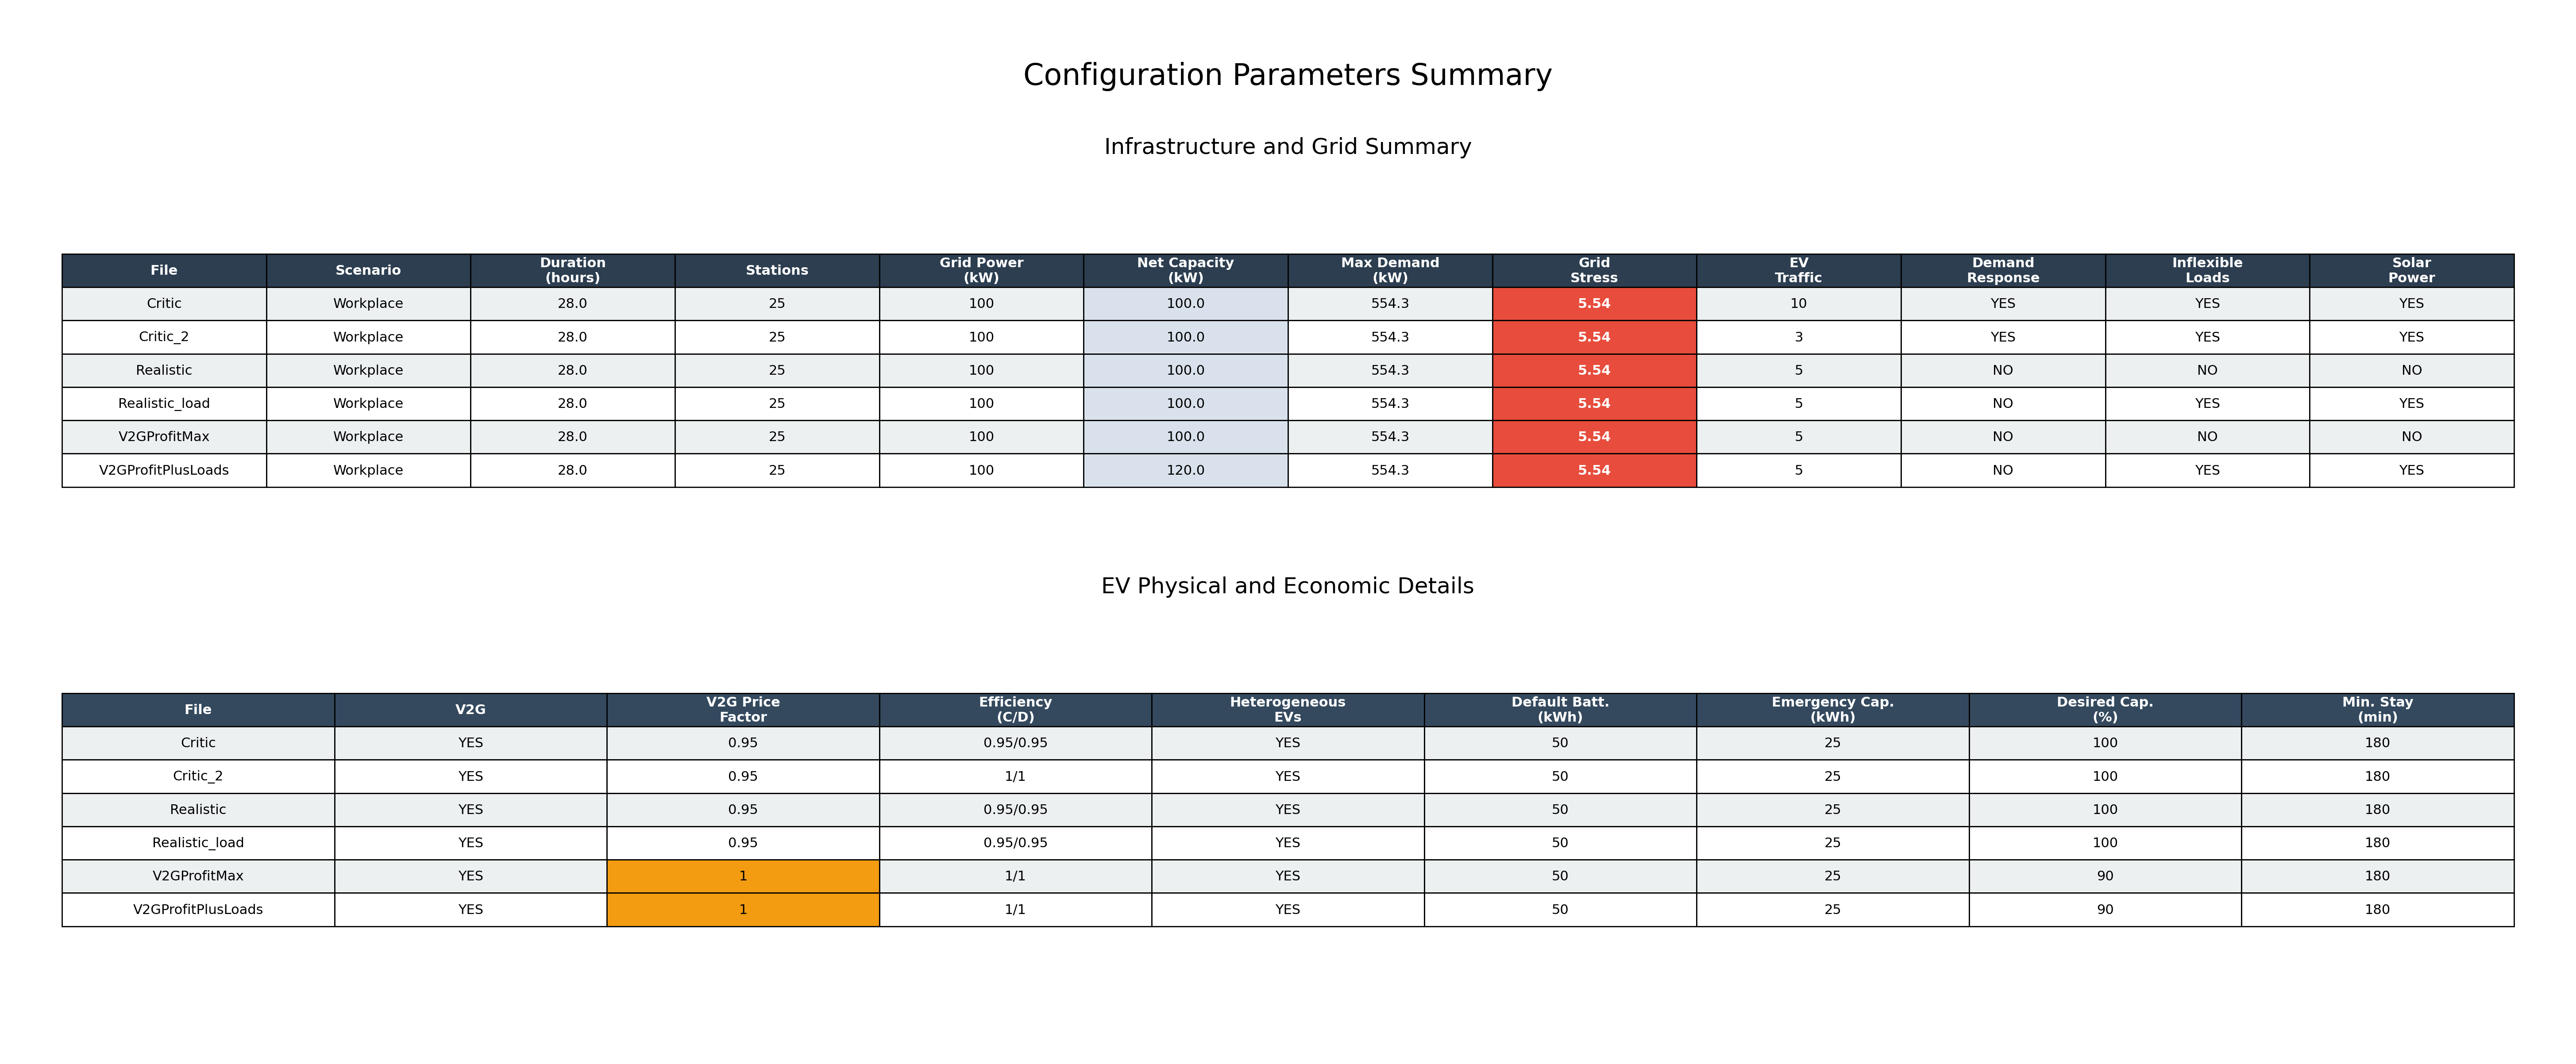
\includegraphics[width=0.9\linewidth]{Configuration_Summary.png}
    \caption{Configuration summary}
    \label{fig:Configuration}
\end{figure}
\noindent
The resulting Figure \ref{fig:Configuration} provides a clear, visual overview of all configuration scenarios, allowing an immediate comparison of grid capacity, EV behavior, and simulation parameters.








\subsection{Scenario 1: Critical Case}


This scenario represents a critical, high-stress condition designed to test the limits and robustness of the control algorithms. It is characterized by high electricity price volatility, creating significant opportunities for V2G arbitrage but also increasing the risk of economic losses. Furthermore, it simulates a high demand for charging, with a large number of EVS present simultaneously, placing a heavy load on the grid infrastructure and increasing the likelihood of transformer overloads. The following plots illustrate the scenario conditions and the comparative performance of the tested algorithms.

\subsubsection{Scenario Conditions}

\begin{figure}[H]
    \centering
    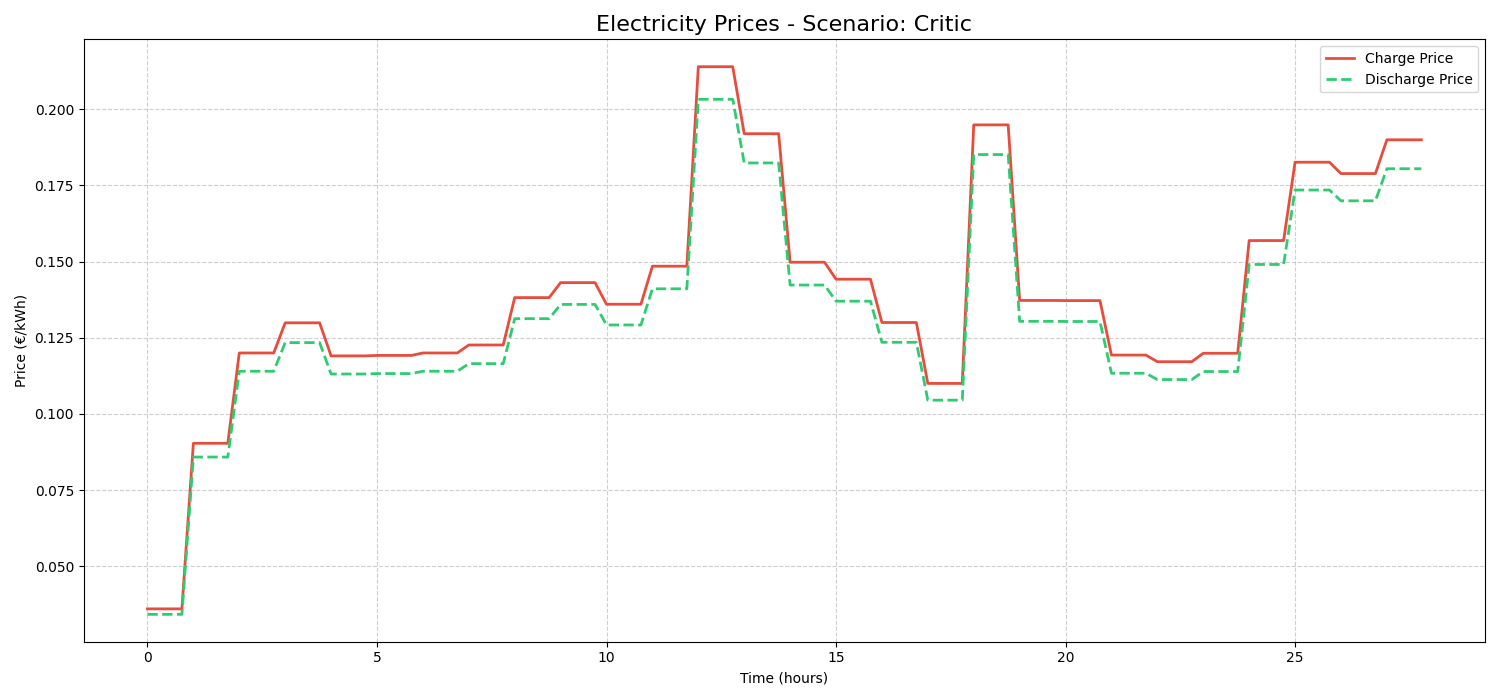
\includegraphics[width=0.9\linewidth]{../results/benchmark_20251025_105855/Critic/electricity_prices_Critic.png}
    \caption{Electricity price profile for the Critical scenario.}
    \label{fig:Critic_prices}
\end{figure}

\begin{figure}[H]
    \centering
    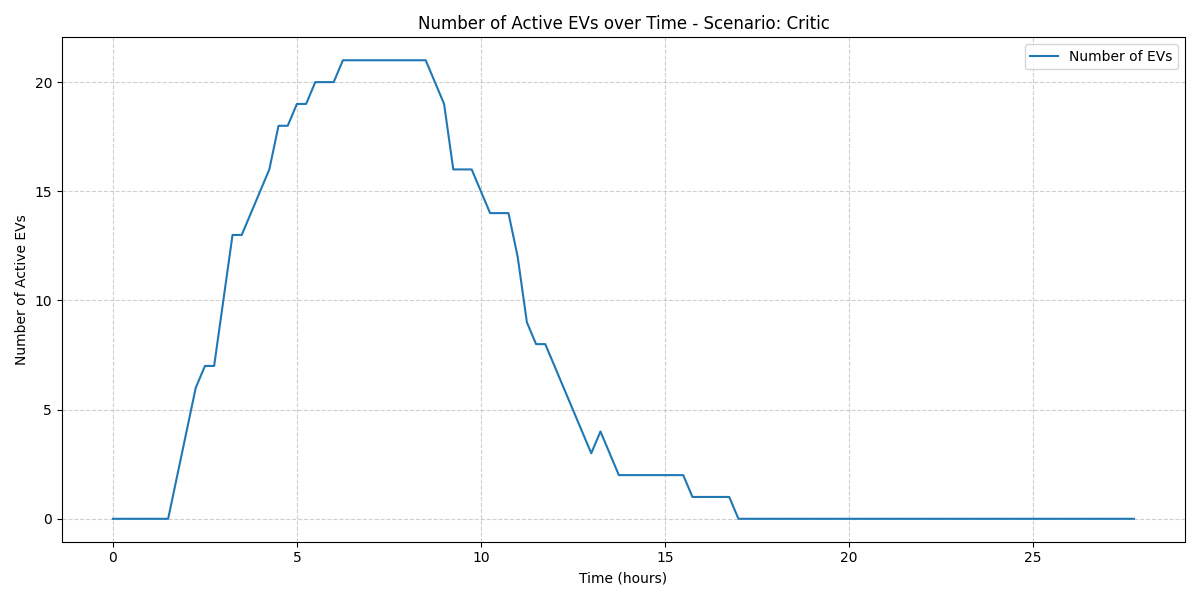
\includegraphics[width=0.9\linewidth]{../results/benchmark_20251025_105855/Critic/ev_presence_Critic.png}
    \caption{Number of EVs present at the charging station over time.}
    \label{fig:Critic_ev_presence}
\end{figure}
\noindent
The scenario \ref{fig:Critic_ev_presence}simulates a high-density environment, leading to significant aggregate demand for power since the spawn multiplier for the critic scenario is very high(1).
\subsubsection{Overall Performance Summary}

\begin{figure}[H]
    \centering
    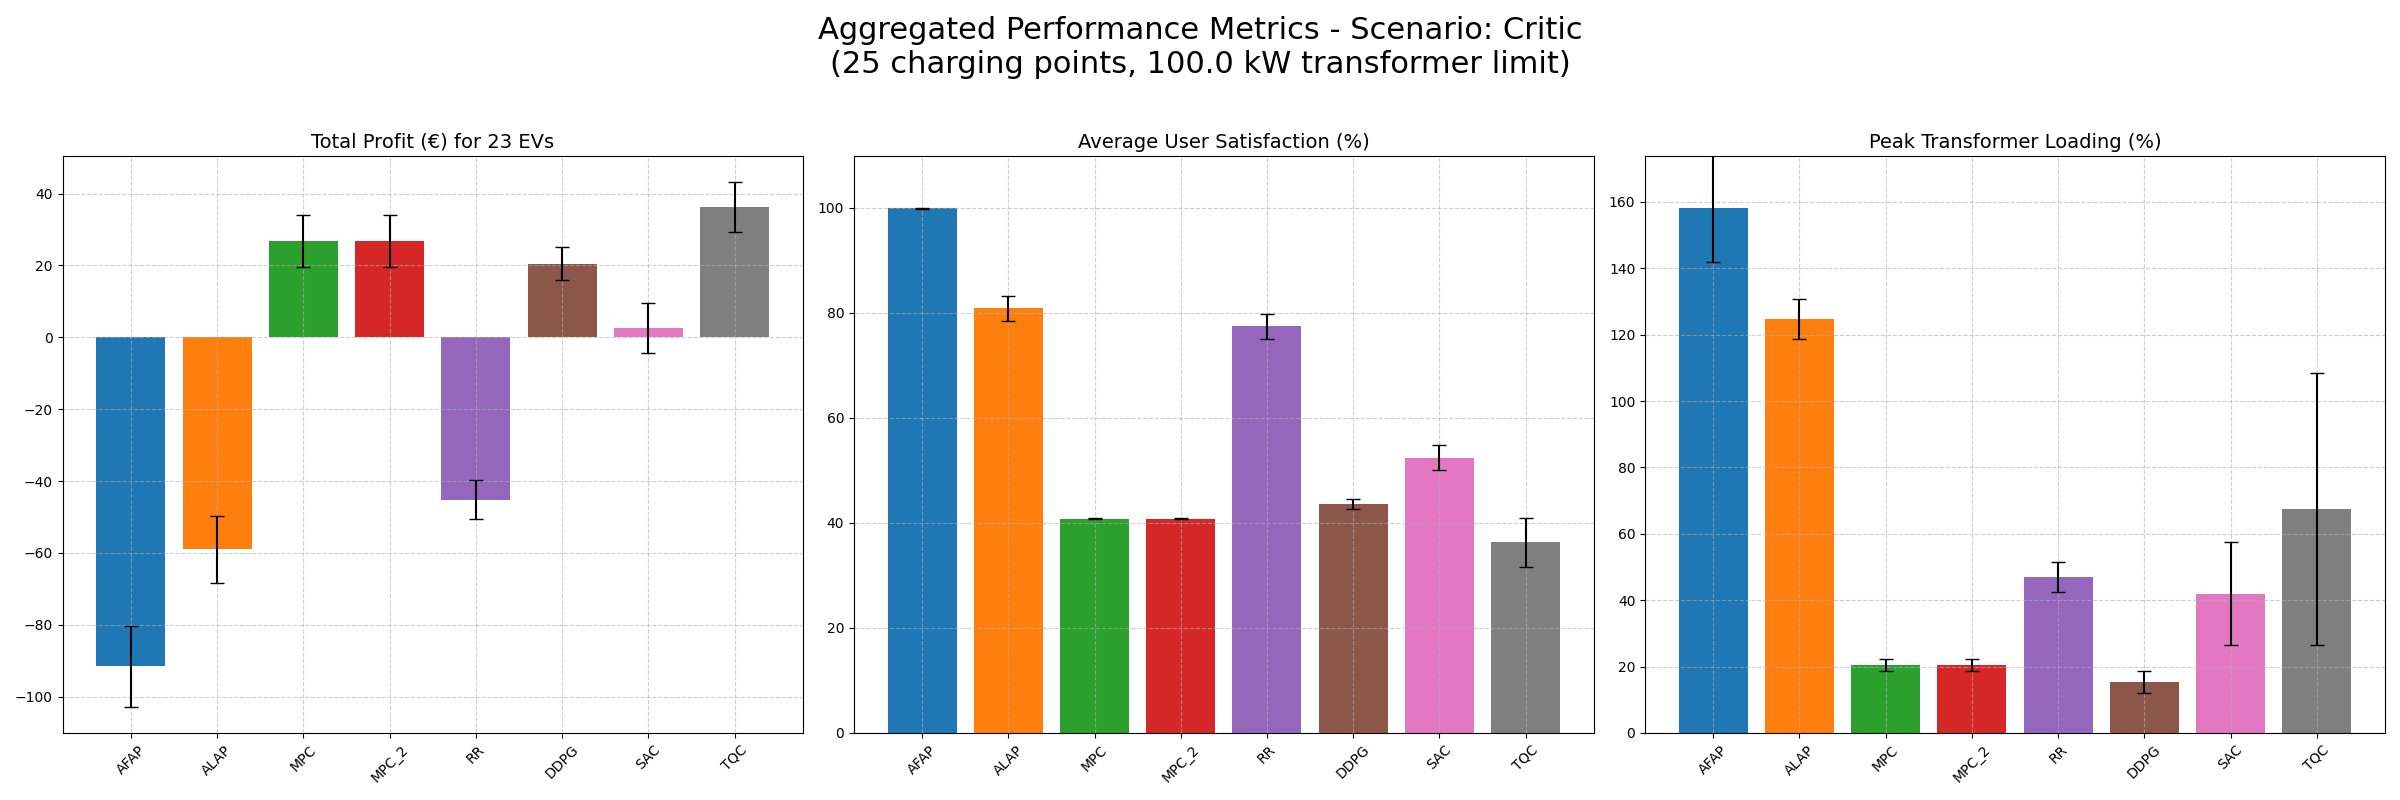
\includegraphics[width=\textwidth]{../results/benchmark_20251025_105855/Critic/performance_summary_Critic.png}
    \caption{Overall performance summary comparing all algorithms across key metrics. }
    \label{fig:Critic_perf_summary}
\end{figure}
\noindent
In this high-stress scenario \ref{fig:Critic_perf_summary}, the TQC and DDPG demonstrate superior profitability, effectively leveraging V2G, but DDPG goes better in the overall metrics better managing the trasformer overload. Heuristic methods like AFAP and ALAP result in significant economic losses and grid overloads.
Both MPC algorithms achieved a good profit but less average users' satisfaction. SAC achieved the best average satisfaction among RL algorithms but fewer profit.
\begin{figure}[H]
    \centering
    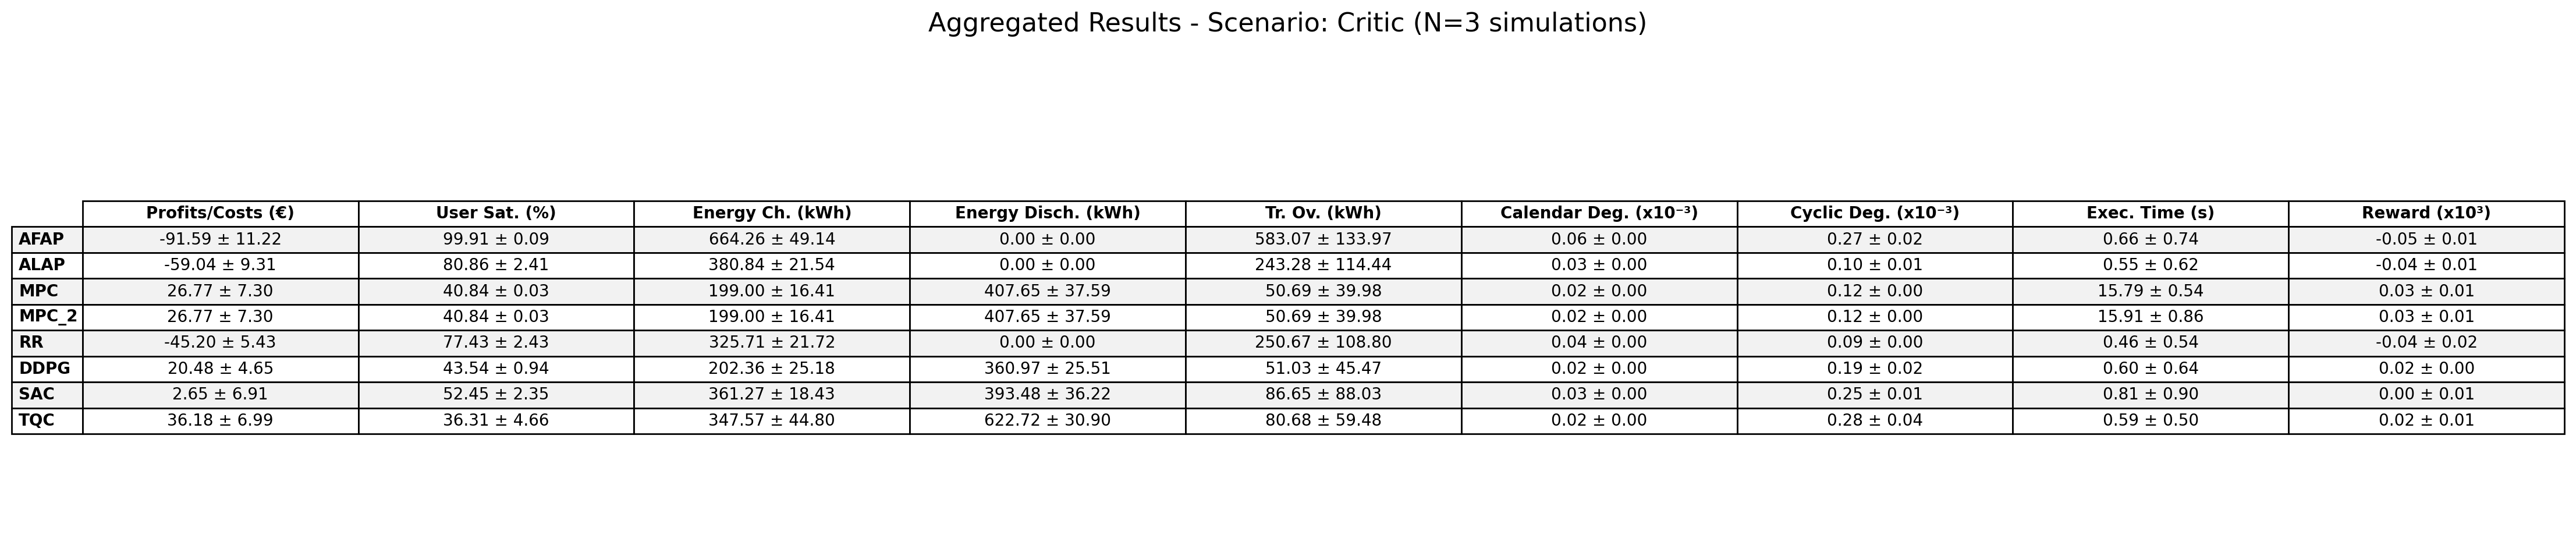
\includegraphics[width=\textwidth]{../results/benchmark_20251025_105855/Critic/summary_table_Critic.png}
    \caption{Tabular summary of performance metrics.}
    \label{fig:Critic_summary_table}
\end{figure}
\noindent
This table \ref{fig:Critic_summary_table} provides the
precise numerical data for Total Profit, User Satisfaction, Grid Overload, and
Battery Degradation, confirming the visual insights from the bar chart.
\begin{figure}[H]
    \centering
    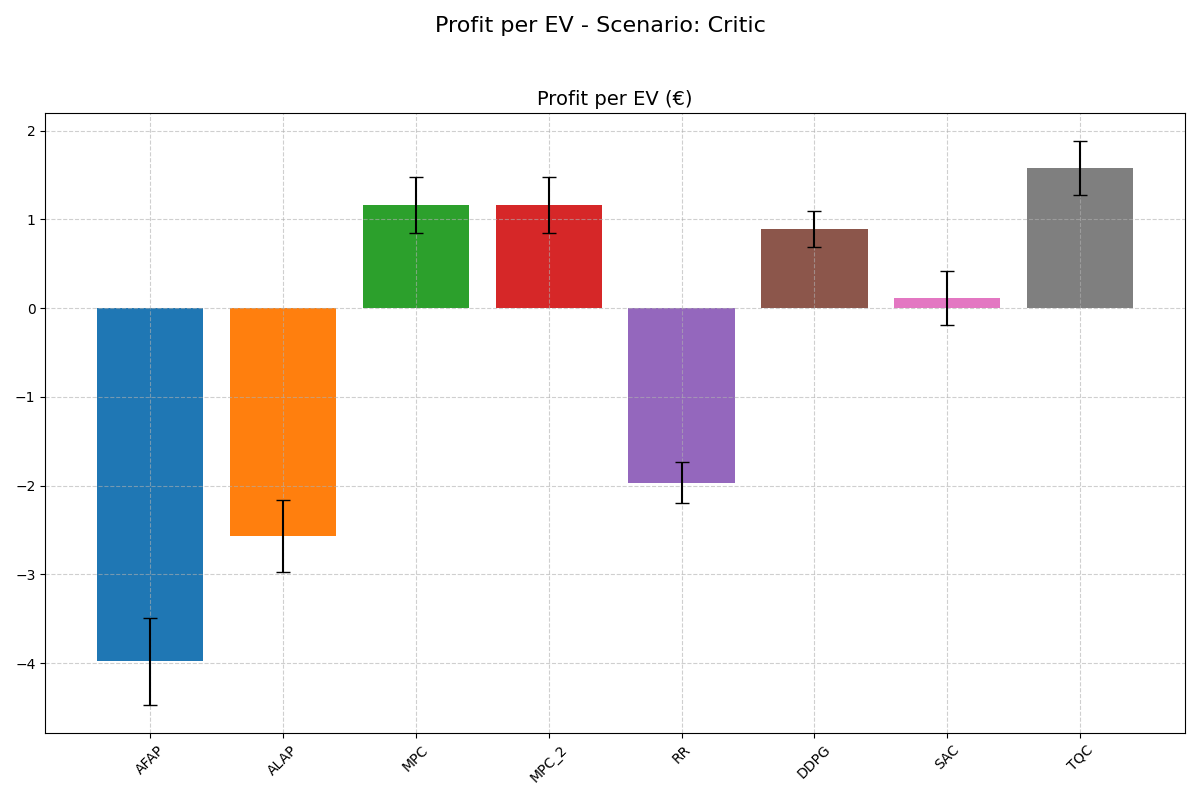
\includegraphics[width=0.9\linewidth]{../results/benchmark_20251025_105855/Critic/profit_per_ev_Critic.png}
    \caption{Average profit generated per EV.}
    \label{fig:Critic_profit_per_ev}
\end{figure}
\noindent
This metric \ref{fig:Critic_profit_per_ev} normalizes the total profit by the number of vehicles served, highlighting the economic efficiency of each control strategy on a per-user basis.
\begin{figure}[H]
    \centering
    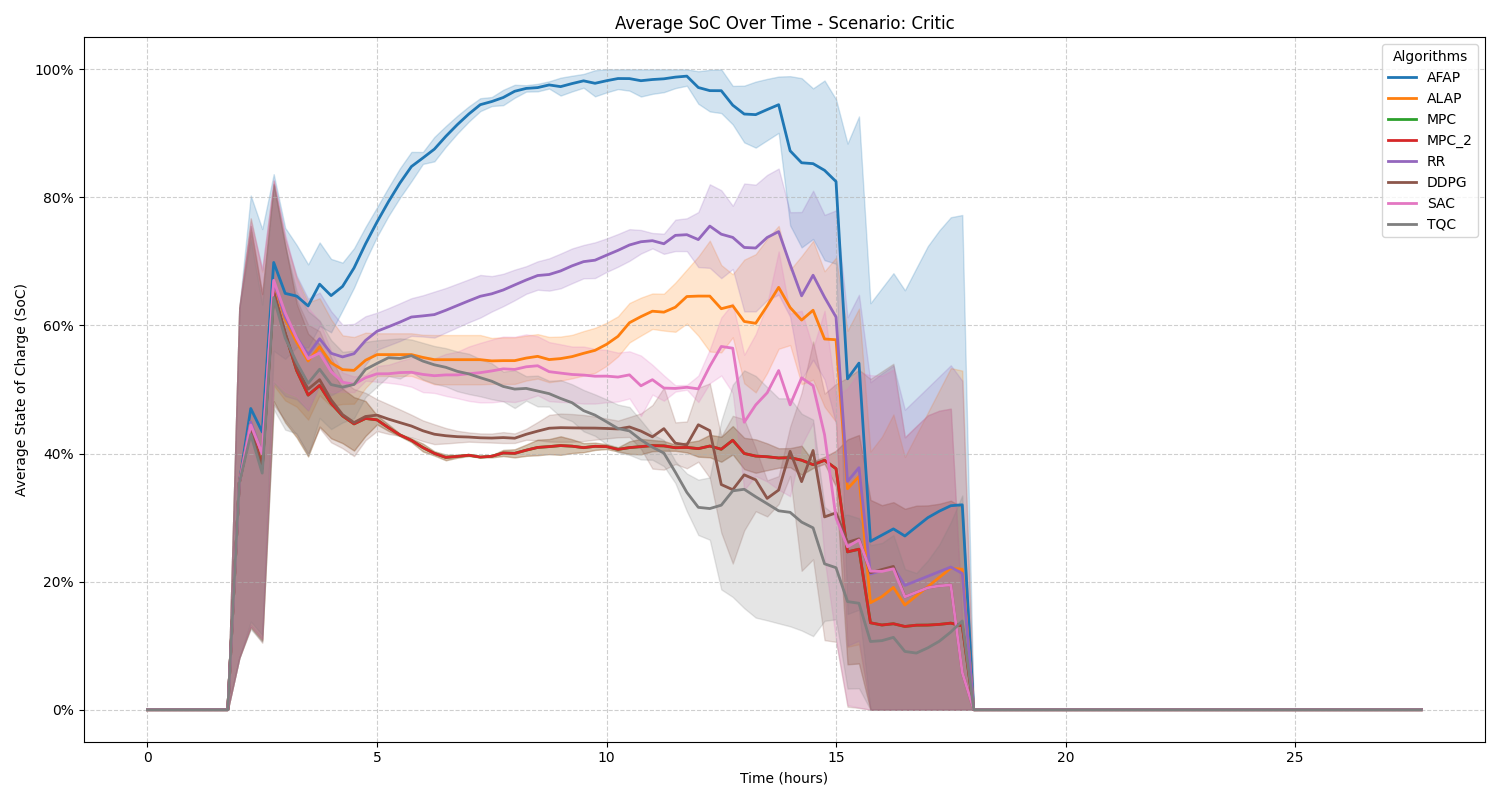
\includegraphics[width=0.9\linewidth]{../results/benchmark_20251025_105855/Critic/average_soc_over_time_Critic.png}
    \caption{Average State of Charge (SoC) of all connected EVs over time.}
    \label{fig:Critic_avg_soc}
\end{figure}
\noindent
As shown in Figure \ref{fig:Critic_avg_soc} RL and MPC agents maintain a lower average SoC during low-price periods to prepare for charging, while heuristics like AFAP charge aggressively upon arrival.
\clearpage
\subsubsection{Grid Impact Analysis}
This subsection analyzes the impact of each algorithm on the grid, focusing on transformer load and overload events.

\begin{figure}[H]
    \centering
    \begin{subfigure}{0.49\textwidth}
        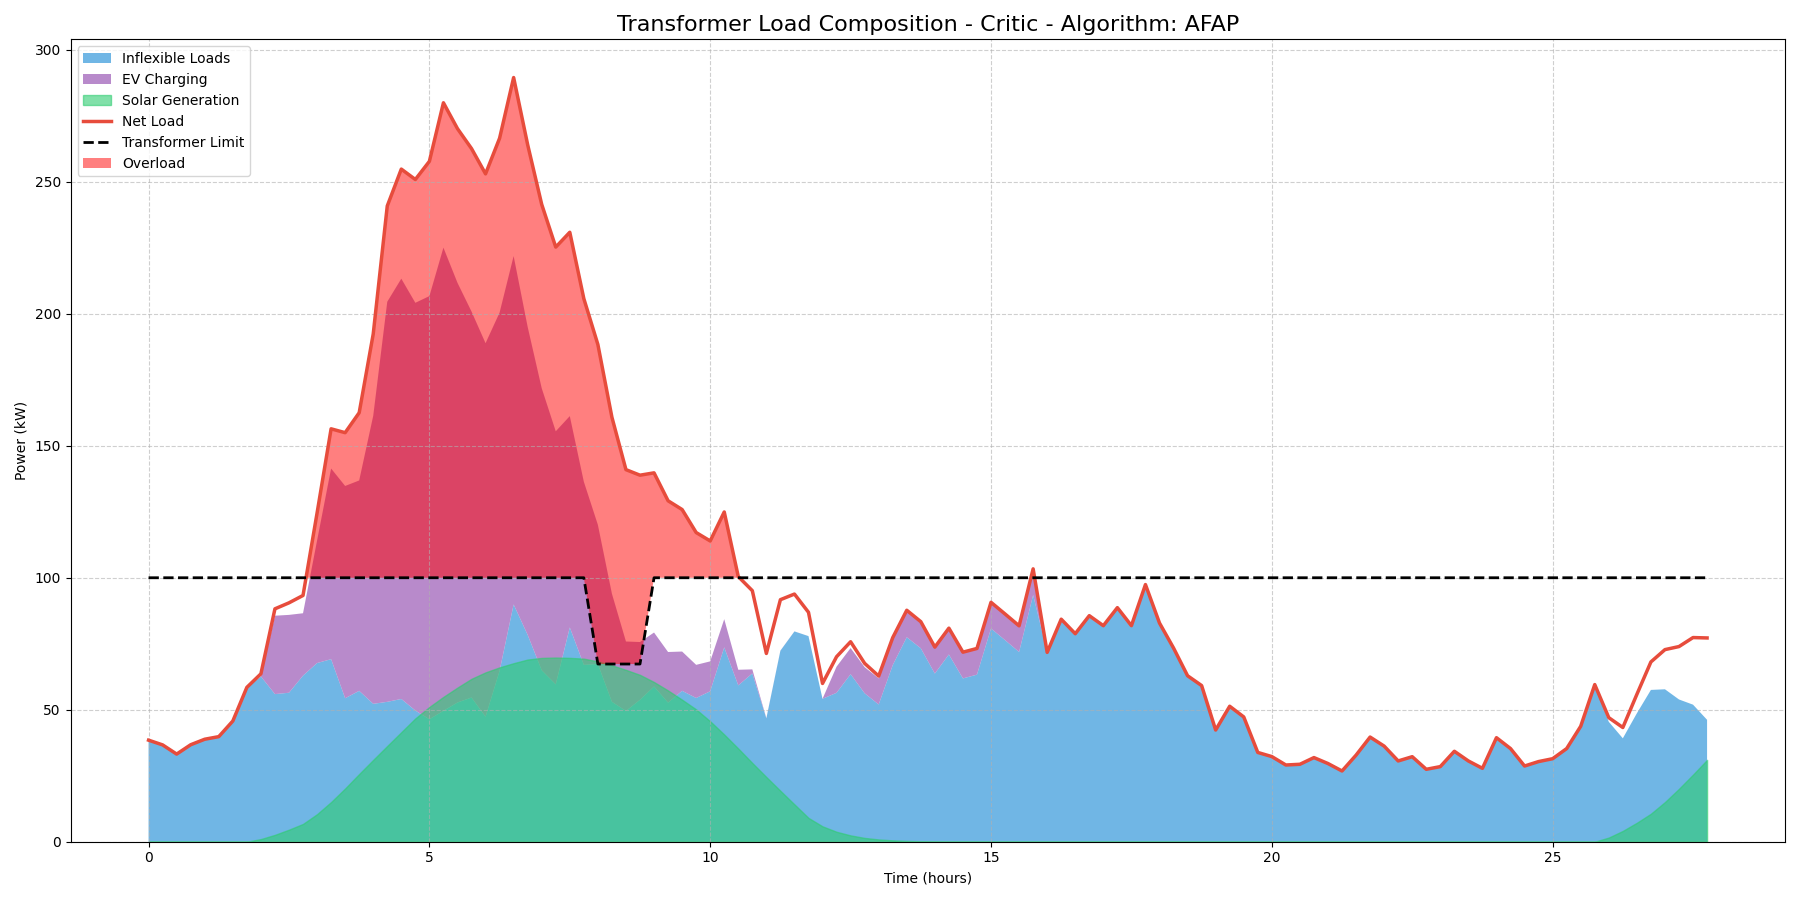
\includegraphics[width=\linewidth]{../results/benchmark_20251025_105855/Critic/overload_composition_Critic_AFAP.png}
        \caption{Overload composition for AFAP algorithm.}
    \end{subfigure}
    \hfill
    \begin{subfigure}{0.49\textwidth}
        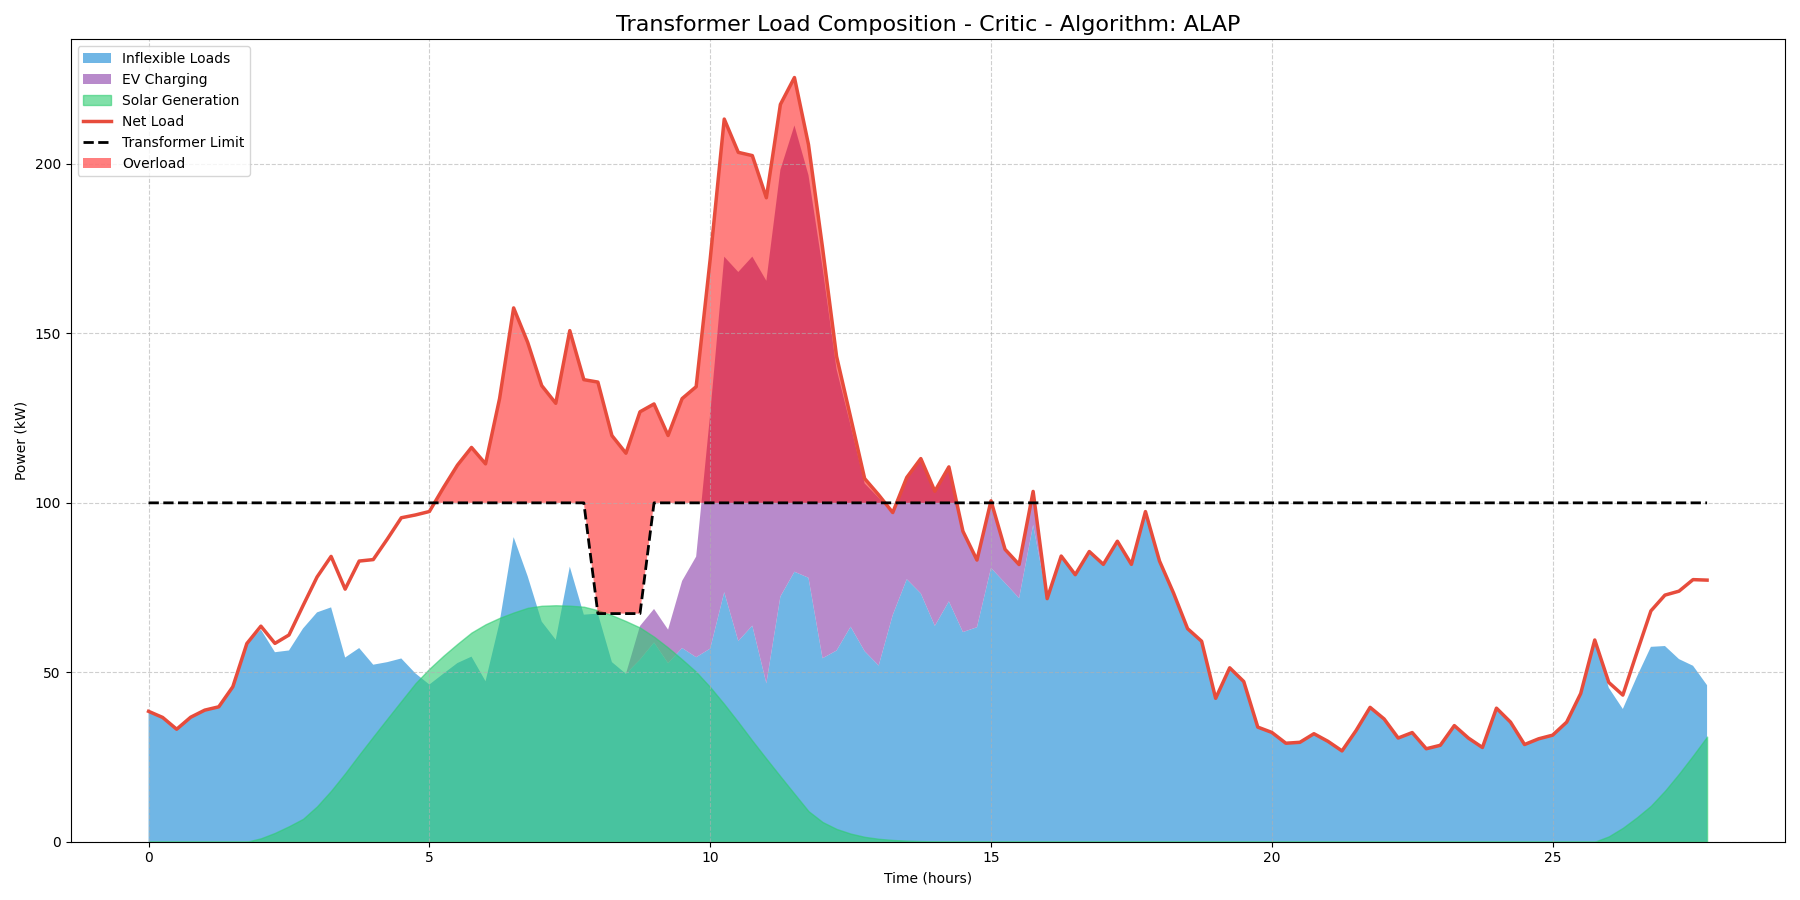
\includegraphics[width=\linewidth]{../results/benchmark_20251025_105855/Critic/overload_composition_Critic_ALAP.png}
        \caption{Overload composition for ALAP algorithm.}
    \end{subfigure}
    \caption{Grid load for heuristic algorithms.}
    \label{fig:Critic_overload_heuristics}
\end{figure}
\noindent
 As shown in Figure \ref{fig:Critic_overload_heuristics} AFAP and ALAP show significant and prolonged periods of transformer overload, as they do not coordinate charging to respect grid limits.
\begin{figure}[H]
    \centering
    \begin{subfigure}{0.49\textwidth}
        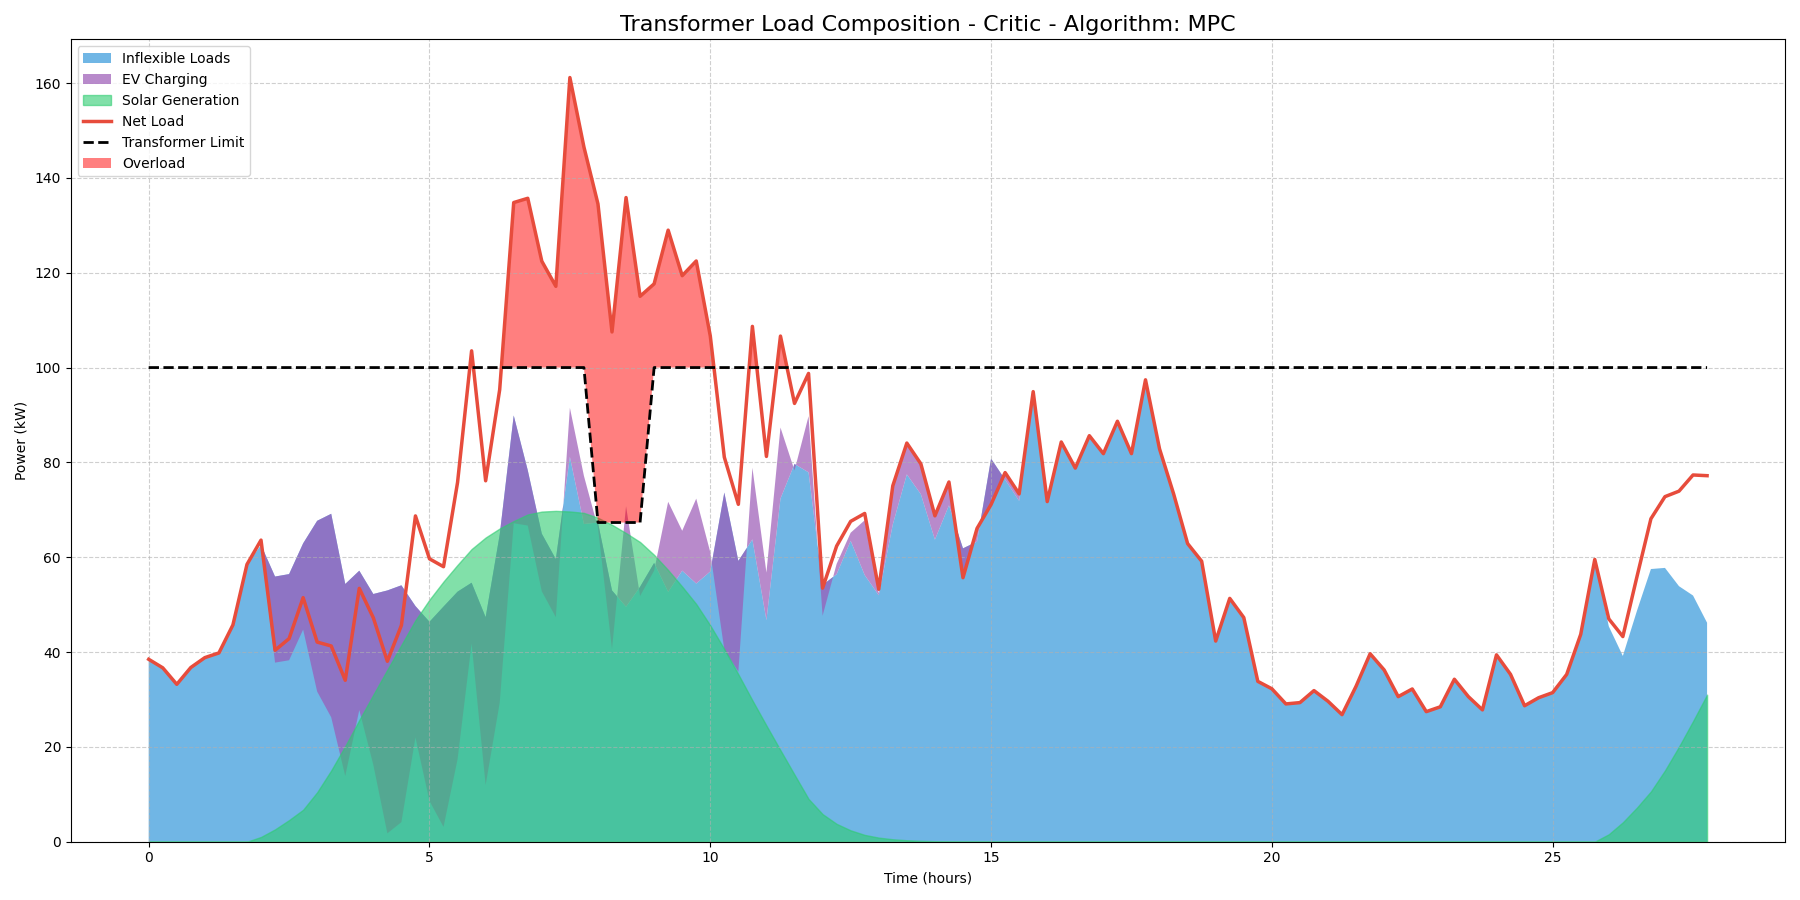
\includegraphics[width=\linewidth]{../results/benchmark_20251025_105855/Critic/overload_composition_Critic_MPC.png}
        \caption{Overload composition for MPC Non-Adaptive algorithm.}
    \end{subfigure}
    \hfill
    \begin{subfigure}{0.49\textwidth}
        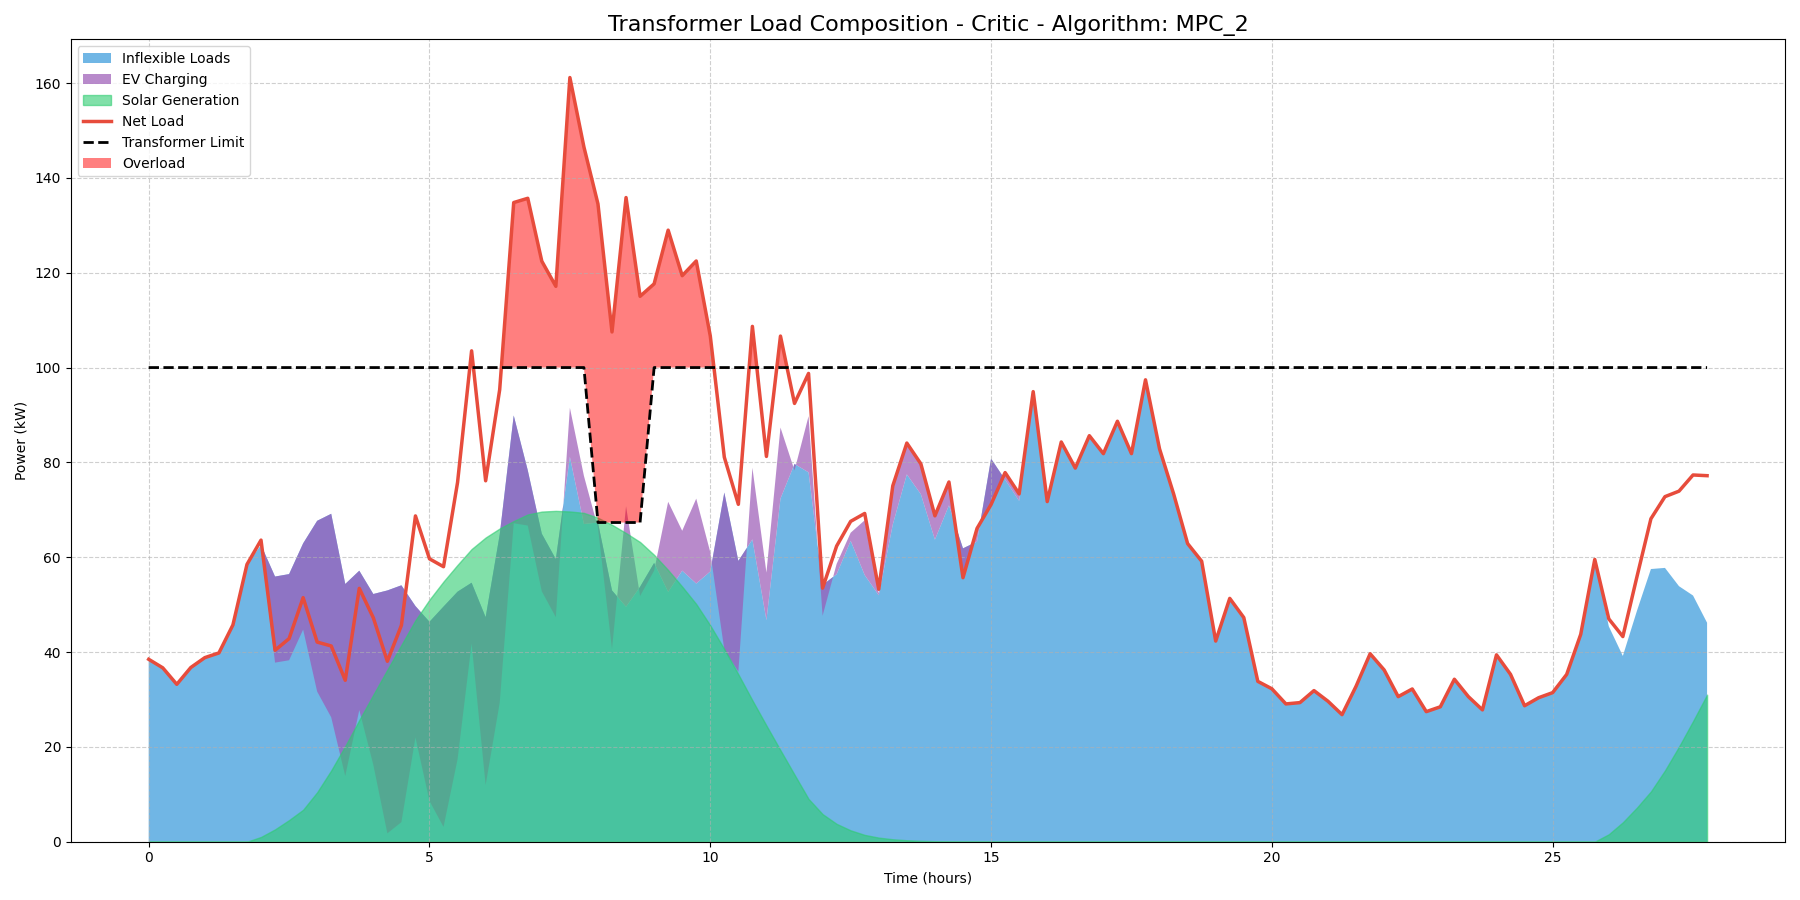
\includegraphics[width=\linewidth]{../results/benchmark_20251025_105855/Critic/overload_composition_Critic_MPC_2.png}
        \caption{Overload composition for MPC Adaptive algorithm.}
    \end{subfigure}
    \caption{Grid load for MPC algorithms. }
    \label{fig:Critic_overload_mpc}
\end{figure}
\noindent
As shown in Figure \ref{fig:Critic_overload_mpc} the MPC controllers are enough effective at preventing overloads.

\begin{figure}[H]
    \centering
    \begin{subfigure}{0.49\textwidth}
        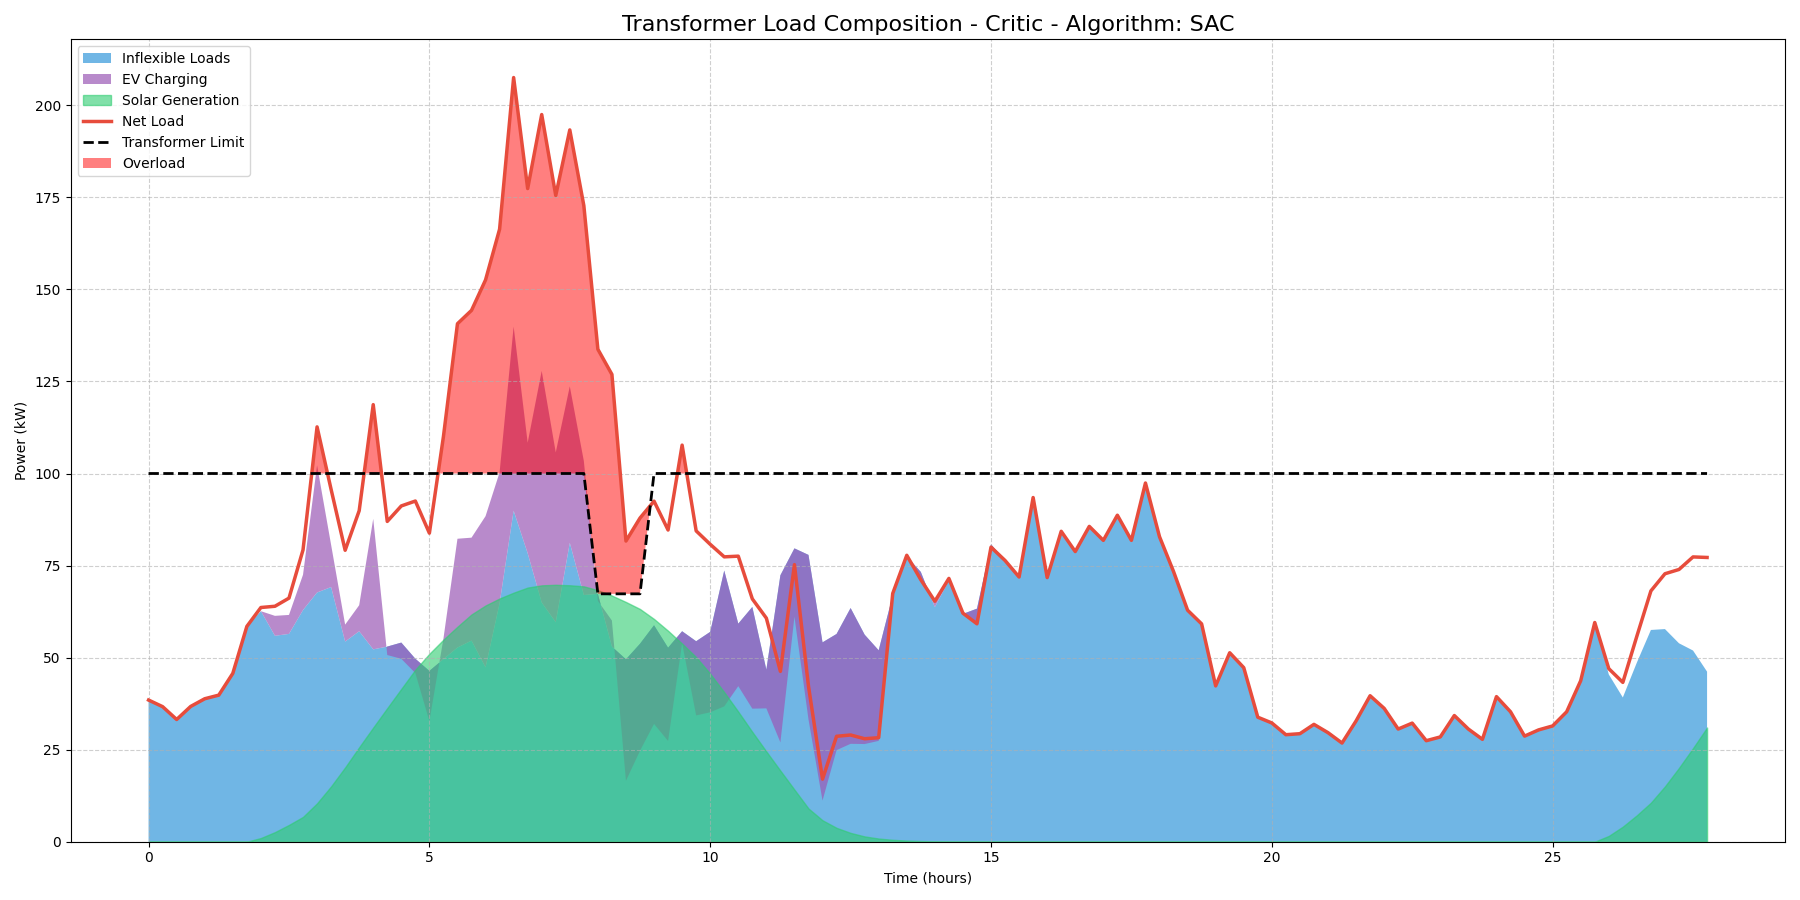
\includegraphics[width=\linewidth]{../results/benchmark_20251025_105855/Critic/overload_composition_Critic_SAC.png}
        \caption{Overload composition for SAC algorithm.}
    \end{subfigure}
    \hfill
    \begin{subfigure}{0.49\textwidth}
        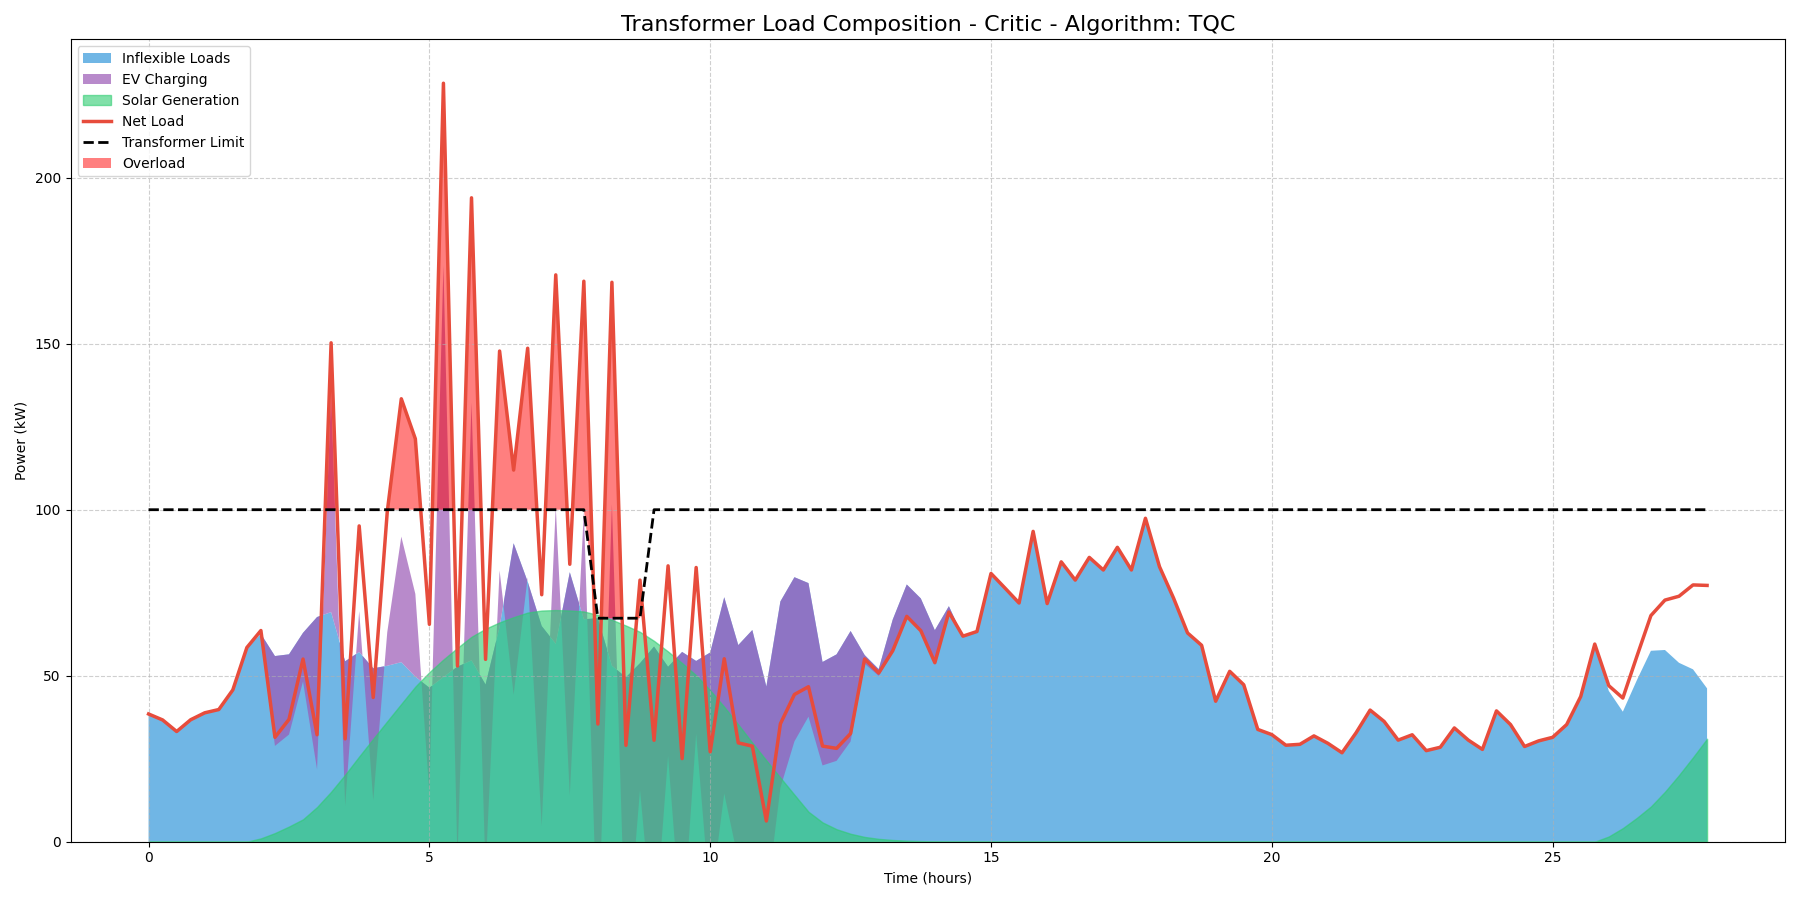
\includegraphics[width=\linewidth]{../results/benchmark_20251025_105855/Critic/overload_composition_Critic_TQC.png}
        \caption{Overload composition for TQC algorithm.}
    \end{subfigure}
    \caption{Grid load for SAC and TQC RL algorithms.}
    \label{fig:Critic_overload_rl1}
\end{figure}

In Figures \ref{fig:Critic_overload_rl1} TQC has a nervous load management with frequent spikes, the SAC agents learn to respect the grid constraints better than TQC.
\begin{figure}[H]
    \centering
 	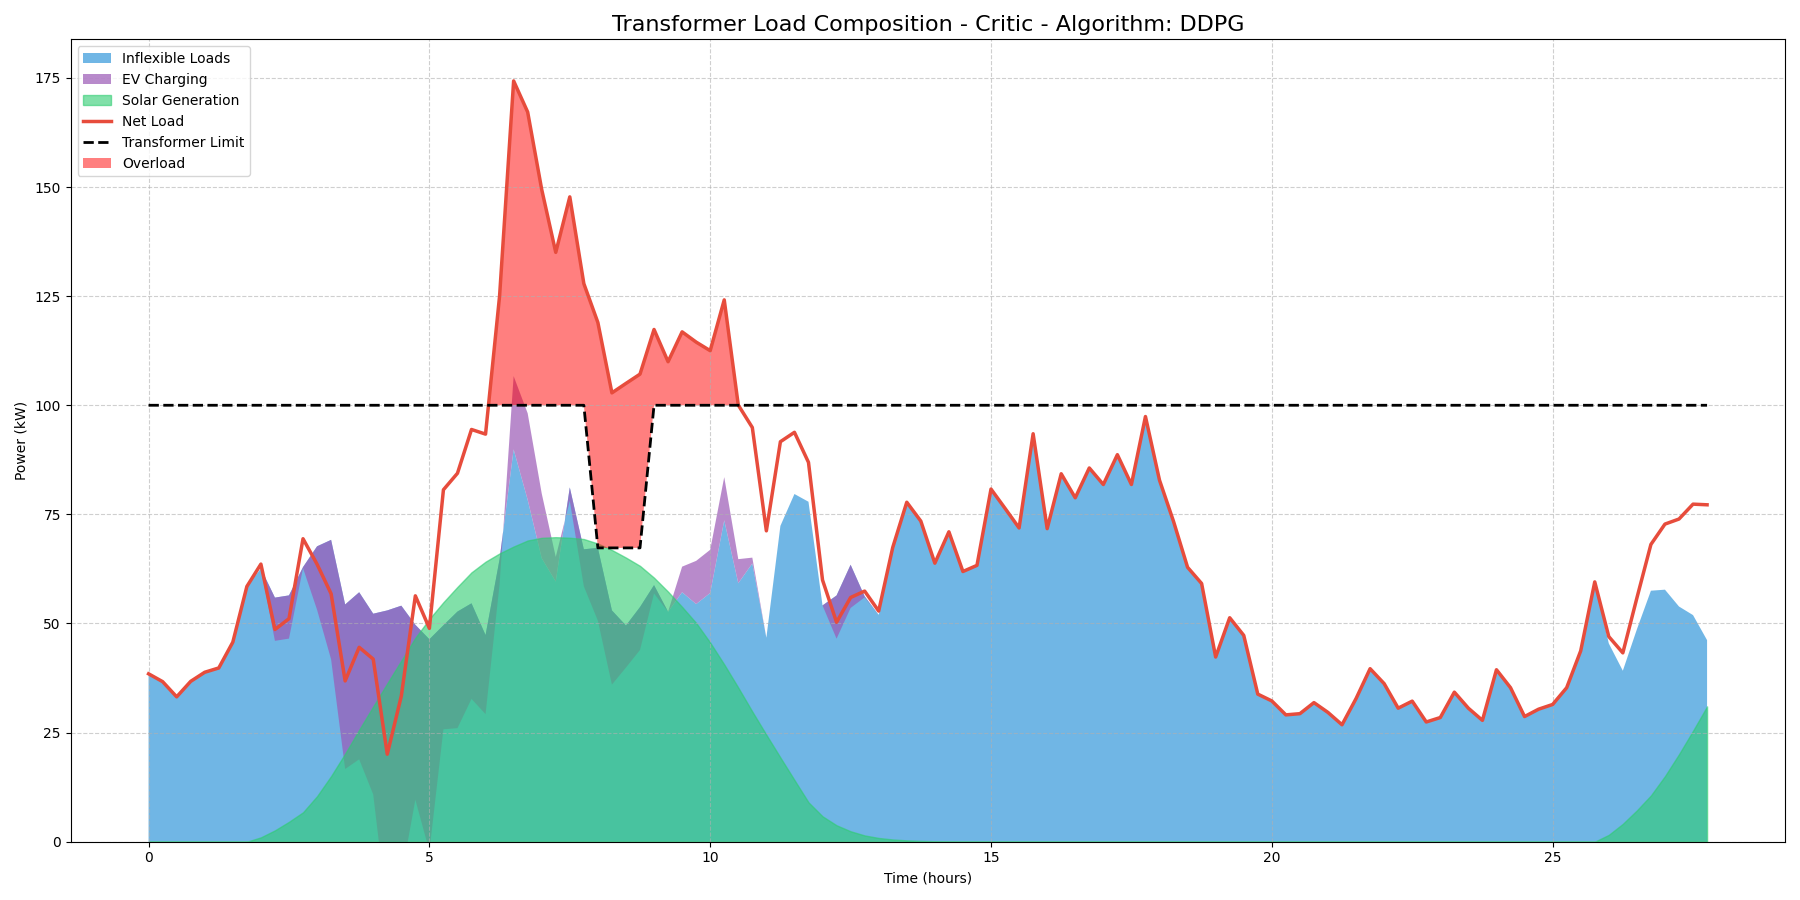
\includegraphics[width=\linewidth]{../results/benchmark_20251025_105855/Critic/overload_composition_Critic_DDPG.png}
        \caption{Overload composition for DDPG algorithm.}
    \caption{Grid load for DDPG algorithm.}
    \label{fig:Critic_overload_rl2}
\end{figure}
\noindent
As shown in Figure \ref{fig:Critic_overload_rl2} DDPG learns to avoid overloads better than other RL algorithms.

\subsubsection{Individual EV Charging Profiles}
The following plots show the detailed charging and discharging behavior for a sample of individual EVs, providing insight into the different strategies employed by each algorithm.

\begin{figure}[H]
    \centering
    \begin{subfigure}{0.49\textwidth}
        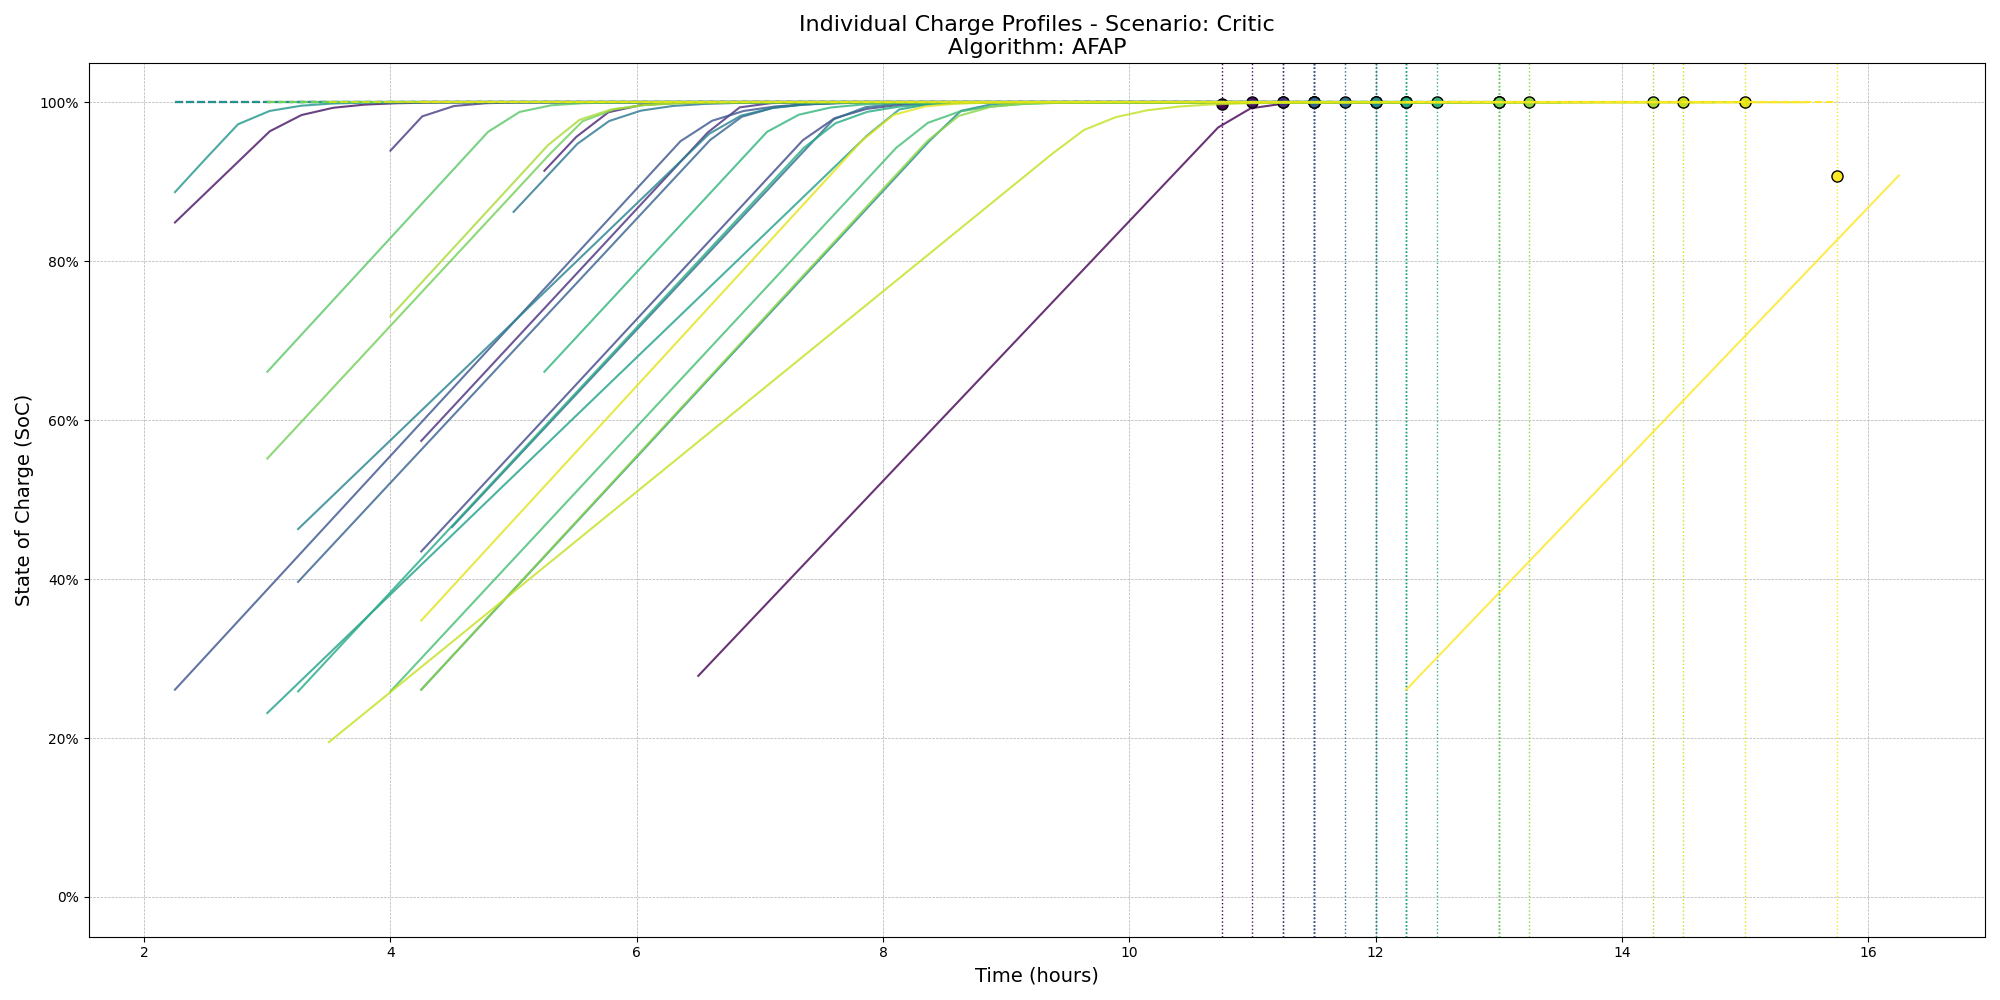
\includegraphics[width=\linewidth]{../results/benchmark_20251025_105855/Critic/individual_ev_profiles_Critic_AFAP.png}
        \caption{Individual ev profiles for AFAP algorithm.}
    \end{subfigure}
    \hfill
    \begin{subfigure}{0.49\textwidth}
        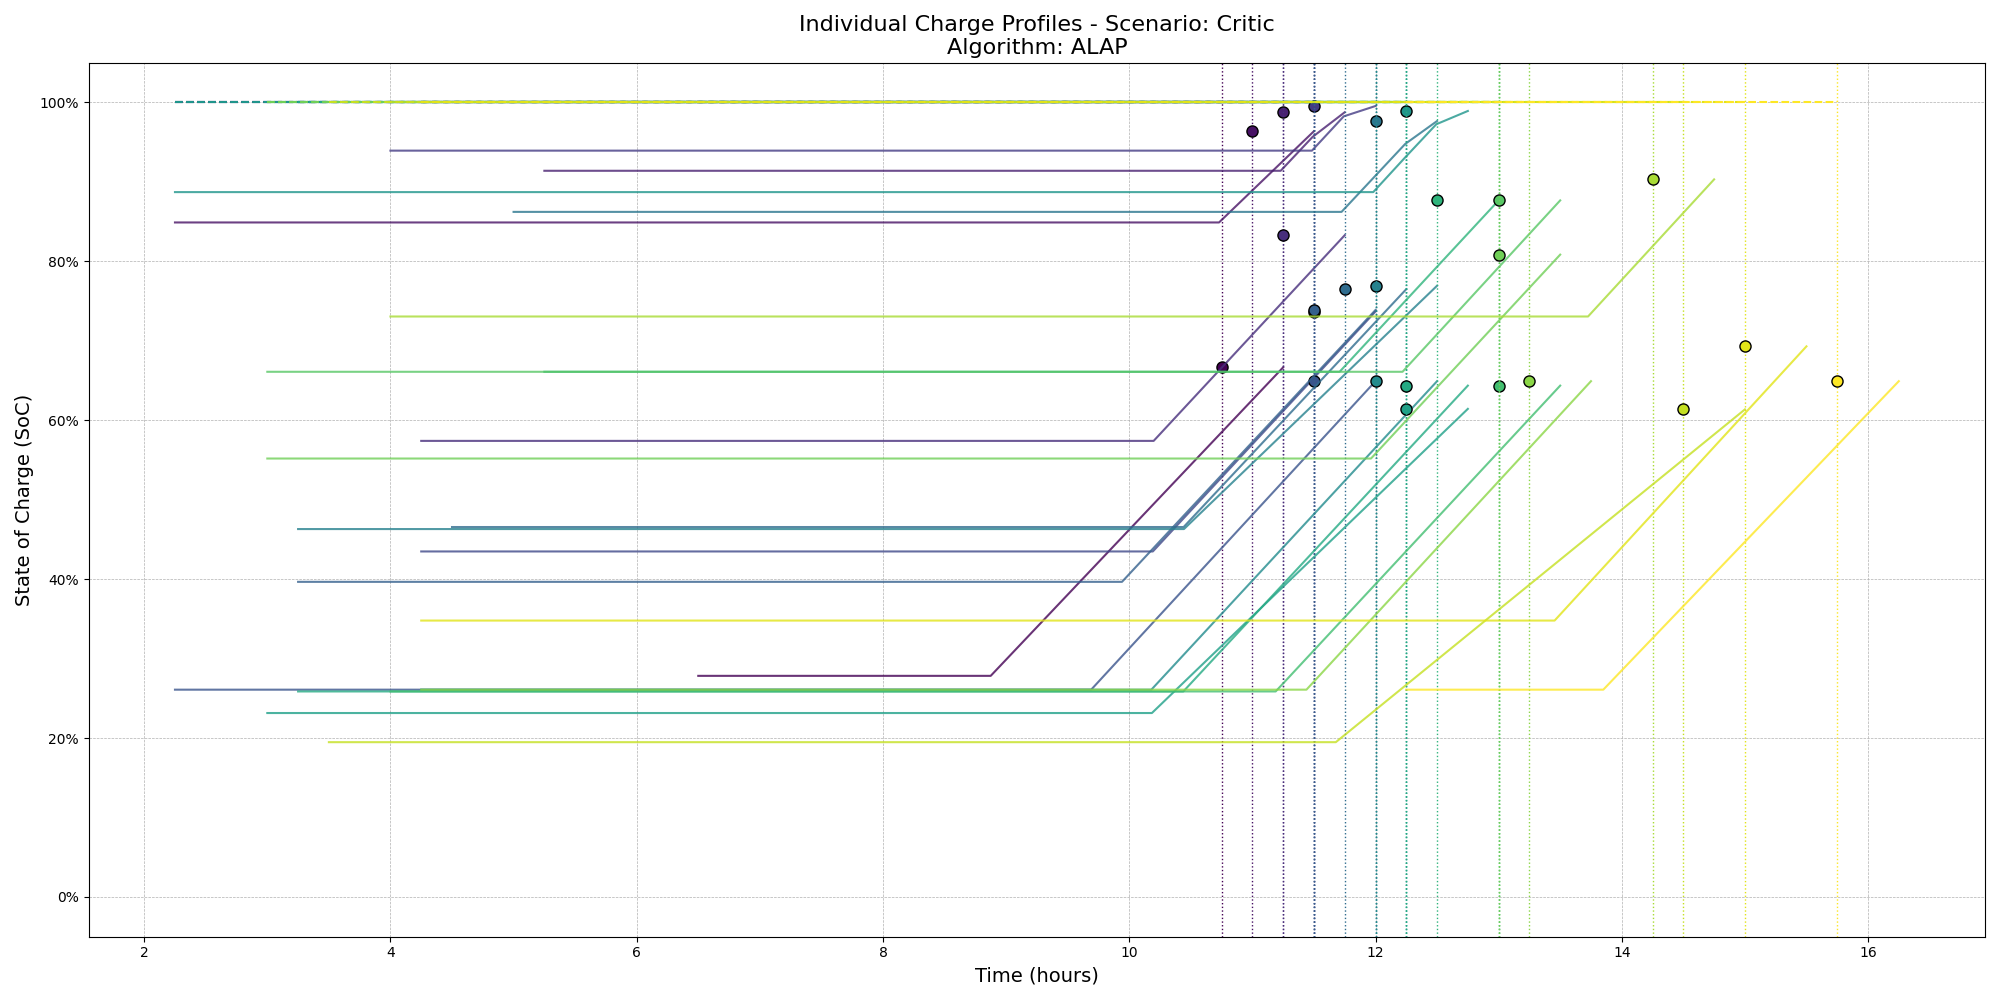
\includegraphics[width=\linewidth]{../results/benchmark_20251025_105855/Critic/individual_ev_profiles_Critic_ALAP.png}
        \caption{Individual ev profiles for ALAP algorithm.}
    \end{subfigure}
    \caption{Individual EV profiles for heuristic algorithms.}
    \label{fig:Critic_profiles_heuristics}
\end{figure}
As shown in Figures in \ref{fig:Critic_profiles_heuristics} AFAP charges immediately upon arrival, while ALAP waits until the last possible moment. Neither strategy responds to price signals.
\begin{figure}[H]
    \centering
    \begin{subfigure}{0.49\textwidth}
        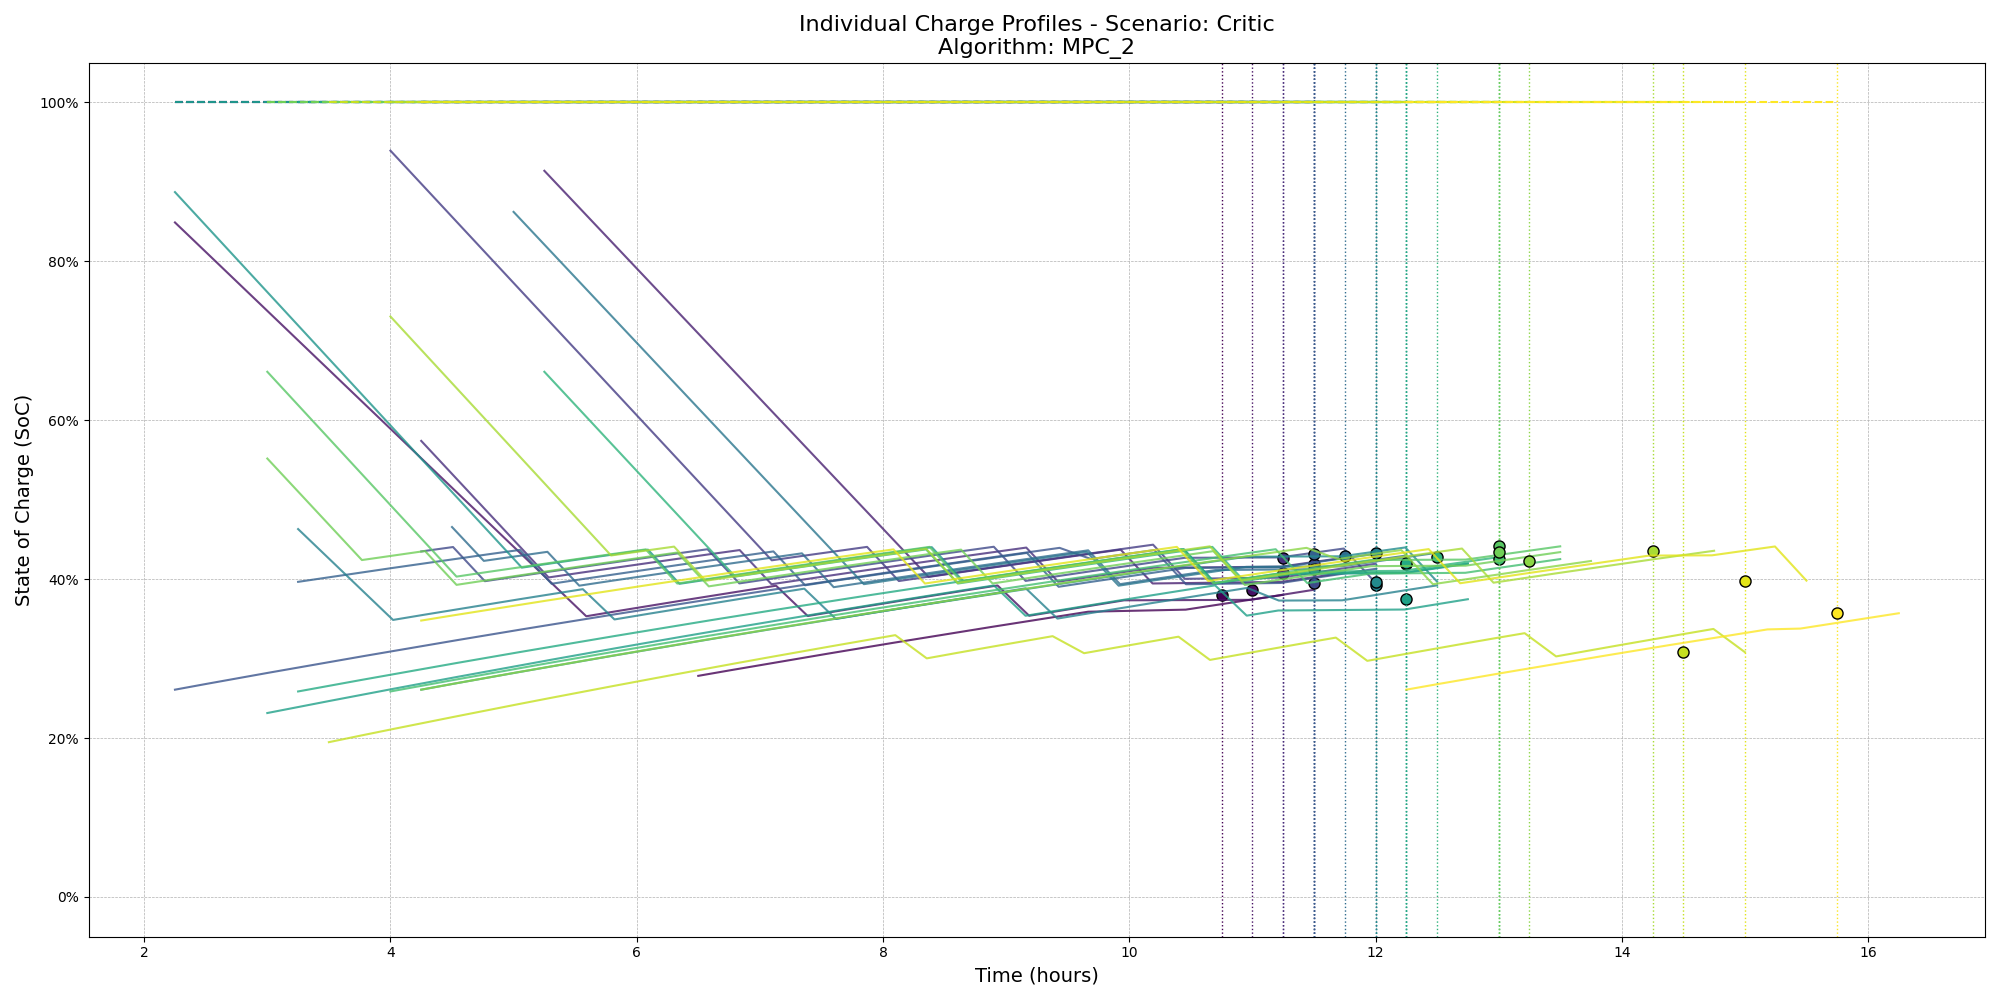
\includegraphics[width=\linewidth]{../results/benchmark_20251025_105855/Critic/individual_ev_profiles_Critic_MPC_2.png}
        \caption{Individual ev profiles for Adaptive MPC: it slightly charges at times, but occasionally exhibits a negative ramp due to discharging.}
    \end{subfigure}
    \hfill
    \begin{subfigure}{0.49\textwidth}
        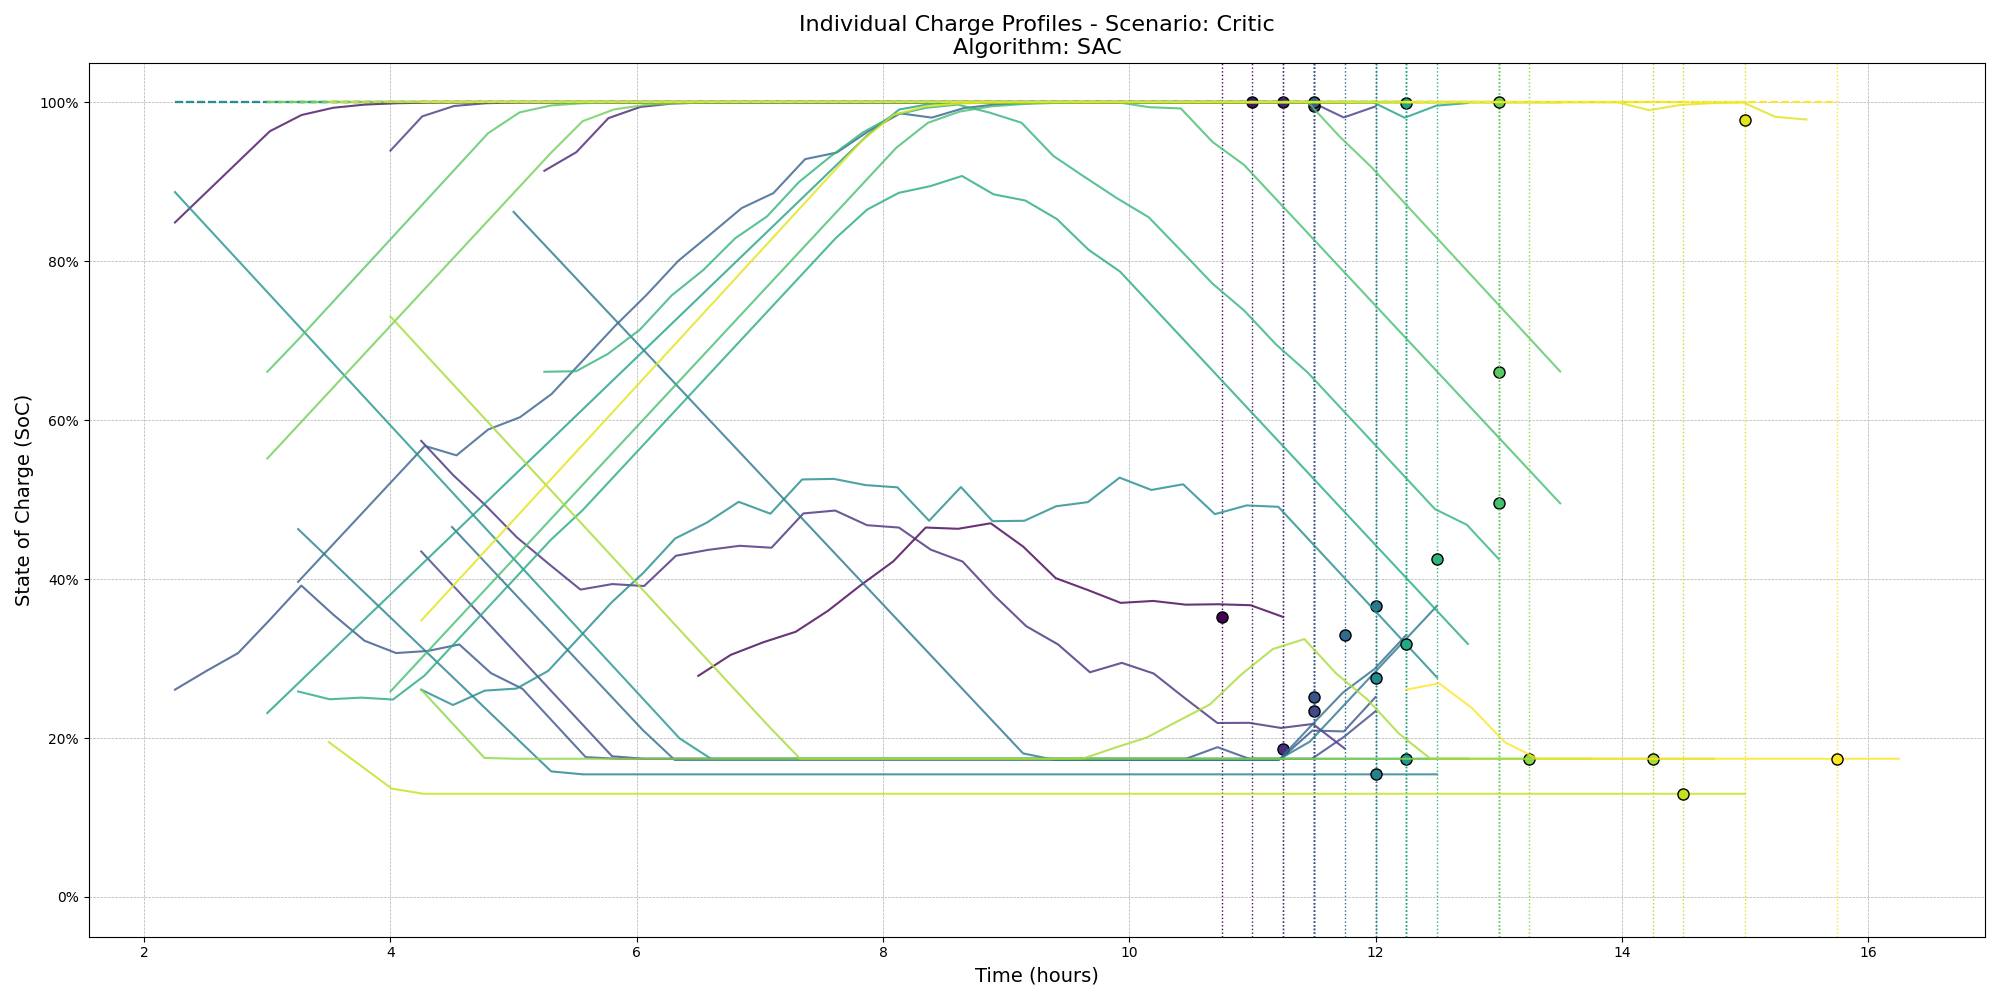
\includegraphics[width=\linewidth]{../results/benchmark_20251025_105855/Critic/individual_ev_profiles_Critic_SAC.png}
        \caption{SAC}
    \end{subfigure}
    \caption{The SAC tends to fully charge some EVs while leaving others partially charged, focusing instead on using certain vehicles to maximize profit.}
    \label{fig:Critic_profiles_advanced}
\end{figure}

\subsection{MPC sensitivity for the Np/Nc ratio}
\begin{figure}[H]
    \centering
    % Prima subfigure
    \begin{subfigure}[b]{0.32\textwidth}
        \centering
        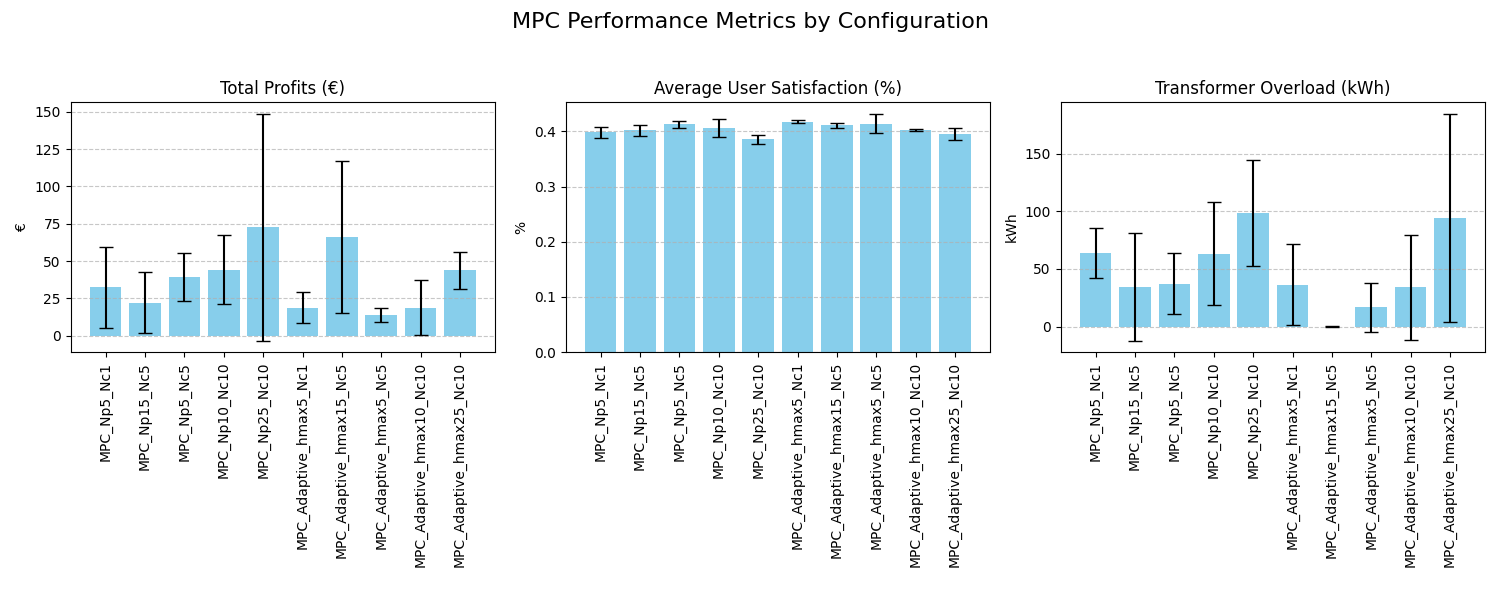
\includegraphics[width=\textwidth]{../sensitivity_analysis_results/Risultati_scelti/mpc_sensitivity_20251023_152425_performance.png}
        \caption{Performance of the algorithms.}
        \label{fig:sub1}
    \end{subfigure}
    \hfill
    % Seconda subfigure
    \begin{subfigure}[b]{0.32\textwidth}
        \centering
        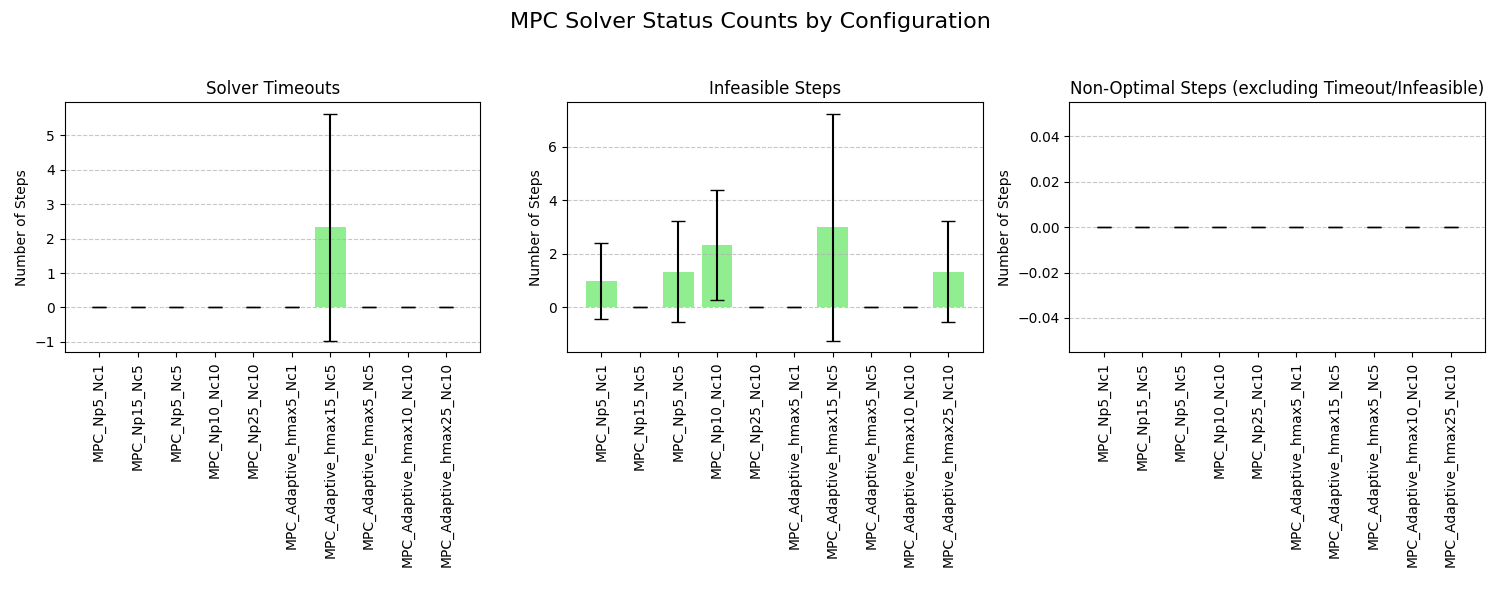
\includegraphics[width=\textwidth]{../sensitivity_analysis_results/Risultati_scelti/mpc_sensitivity_20251023_152425_solver_status.png}
        \caption{Solver status.}
        \label{fig:sub2}
    \end{subfigure}
    \hfill
    % Terza subfigure
    \begin{subfigure}[b]{0.32\textwidth}
        \centering
        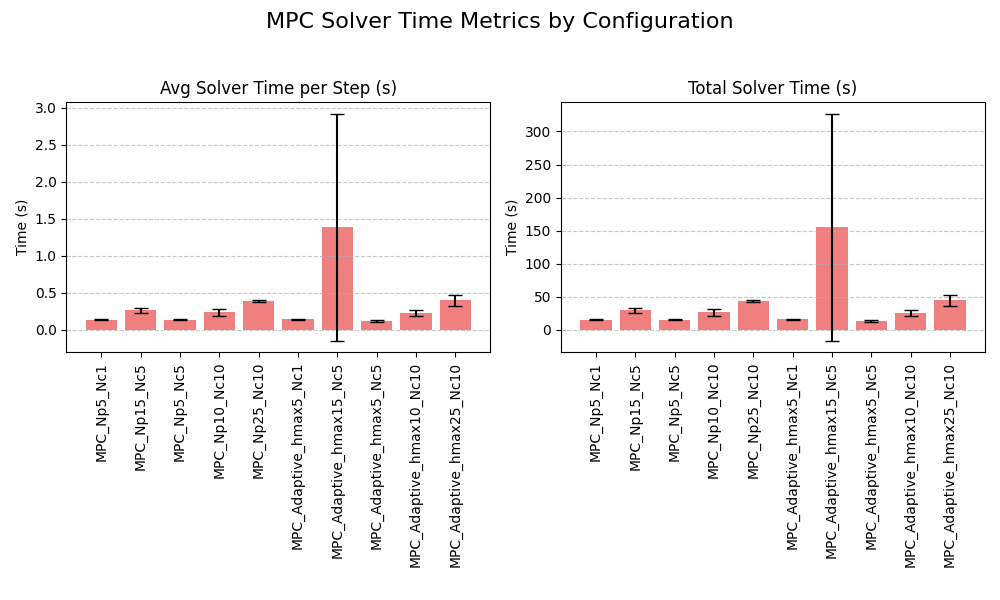
\includegraphics[width=\textwidth]{../sensitivity_analysis_results/Risultati_scelti/mpc_sensitivity_20251023_152425_solver_time.png}
        \caption{Solver time.}
        \label{fig:sub3}
    \end{subfigure}
    
    \caption{MPC sensivity}
    \label{fig:tre_subfigures}
\end{figure}
With this sensitivity analysis performed in the Figures \ref{fig:tre_subfigures}, we can conclude that increasing the 
N\_p/N\_c ratio may improve profit but does not enhance average satisfaction. 
The overload remains zero, which is naturally a result of the high utilization 
of V2G and, consequently, the higher profit.
\\
\noindent
For the adpative MPC we can understand how the algorithm change adaptively through time from Figure \ref{fig:adaptive}.
\begin{figure}[H]
       \centering
       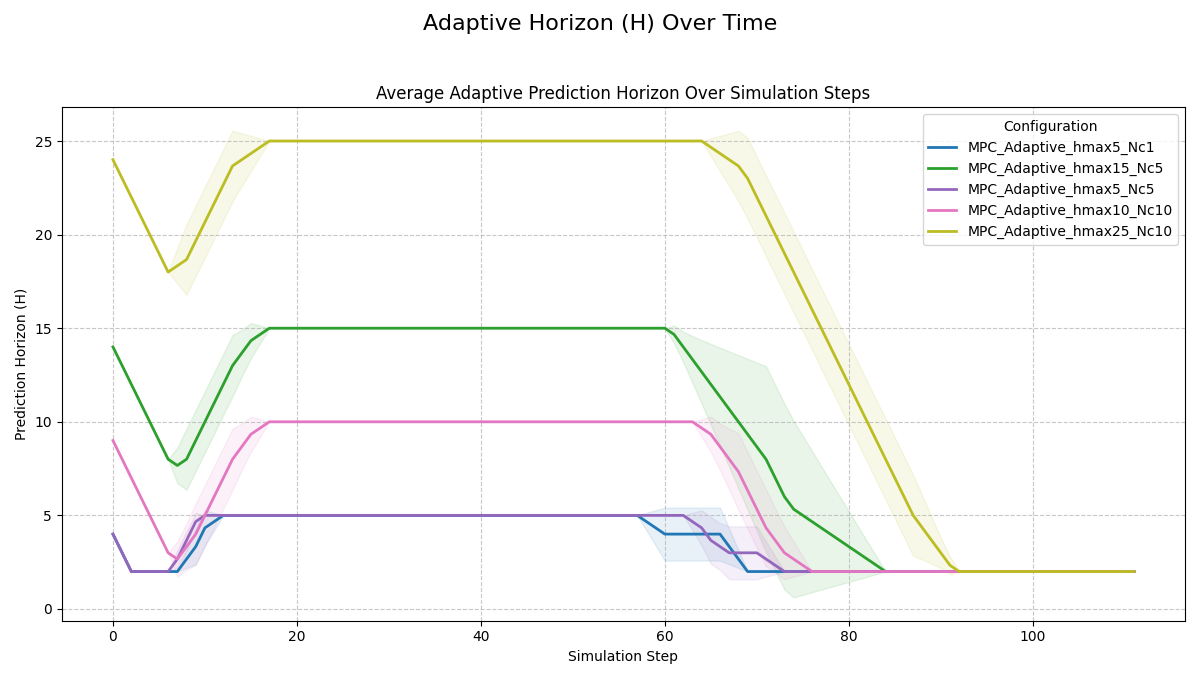
\includegraphics[width=0.8\linewidth]{../sensitivity_analysis_results/Risultati_scelti/mpc_sensitivity_20251023_152425_adaptive_horizon.png}
       \caption{Adaptive horizon.}
       \label{fig:adaptive}
\end{figure}

%\subsection{Scenario 2: Realistic Case}
% TODO: Add analysis and plots for the Realistic scenario.

%\subsection{Scenario 3: Realistic Load Case}
% TODO: Add analysis and plots for the Realistic Load scenario.

%\subsection{Scenario 4: V2G Profit Maximization}
% TODO: Add analysis and plots for the V2GProfitMax scenario.

%\subsection{Scenario 5: V2G Profit with Load Balancing}
% TODO: Add analysis and plots for the V2GProfitPlusLoads scenario.
